\begin{chapterIntro}
This section introduces a high-level overview for the earth system middleware (ESDM) and discusses the architecture according to the 4+1 model (refer to \Cref{sec:about 4+1}).
\Cref{sec: viewpoints/logical} starts with an architecture overview and introduces the core components and their relation to wide spread technologies related to I/O in earth system software.
\Cref{sec: viewpoints/logical} covers the logical view, i.e, multiple aspects that affect how the ESDM operates and which semantics apply internally as well as externally to users/software using the ESDM.
In particular, this includes the responsibilities of key components, the underlying data model and operations to manipulate the data including a mechanism to manage epochs.
In \Cref{sec: viewpoints/physical}, the components are related to their physical location within the hardware and software stacks.
\Cref{sec: viewpoints/process}, discusses active components and processes required by the ESDM and how they interact when working concurrently.
%\Cref{sec: viewpoints/development}, provides the development view and names required interfaces and how to represent information about and within the data model.
\end{chapterIntro}


%%%%%%%%%%%%%%%%%%%%%%%%%%%%%%%%%%%%%%%%%%%%%
\section{Logical View: Component Overview}
\label{sec: viewpoints/logical}


The architecture overview provides only a brief description of the core components of the ESDM.
We will refine the preliminary description of this document while we are building the prototype.
While this document provides an overview of the ultimate system, within the ESiWACE project we will only be able to build a prototype for the central pieces.
We seek to demonstrate the benefit of the middleware for the community to sustain development towards the presented vision.
For more detailed descriptions in particular for the backends refer to \Cref{chap:components and backends}.


%%%%%%%%%%%%%%%%%%%%%%%%%%%%%%%%%%%%%%%%%%%%%%%%%%%%%%%%%%%%%%%%%%%%%%%%%%%%%%%
\paragraph {Problem Summary}
The ESD middleware has been designed to deal with the fact that existing  data
libraries for standardised data description and optimised I/O such as NetCDF,
HDF5 and GRIB do not have suitable performance portable optimisations which
reflect current data intensive system architectures and deliver cost-effective,
acceptable data access bandwidth, latency and data durability.

%%%%%%%%%%%%%%%%%%%%%%%%%%%%%%%%%%%%%%%%%%%%%%%%%%%%%%%%%%%%%%%%%%%%%%%%%%%%%%%
\paragraph {The ESD Middleware}
To address these issues of performance portability, and exploiting exiting shared, interoperable interfaces, based on open standards, we have designed the \textit{Earth System Data (ESD)} middleware (ESDM in short), which:
\begin{enumerate}
	\item understands application data structures and scientific metadata, which lets us expose the same data via different APIs;
	\item maps data structures to storage backends with different performance characteristics based on site specific configuration informed by a performance model;
	\item yields best write performance via optimised data layout schemes that utilise elements from log-structured file systems;
	\item provides relaxed access semantics, tailored to scientific data generation for independent writes, and;
	\item includes a FUSE module which will provide backwards compatibility through existing file formats with a configurable namespace based on scientific metadata.
\end{enumerate}

Together these allow storing small and frequently accessed data on node-local storage, while serialising multi-dimensional data onto multiple storage backends -- providing fault-tolerance and performance benefits for various access patterns at the same time.
Compact-on-read instead of garbage collection will additionally optimise and replicate the data layout during reads via a background service.
Additional tools allow data import/export for exchange between sites and external archives.

The ESDM aids the interests of stakeholders: developers have less burden to provide system specific optimisations and can access their data in various ways.
Data centres can utilise storage of different characteristics.

\bigskip


\begin{figure}[bp]
	\centering
	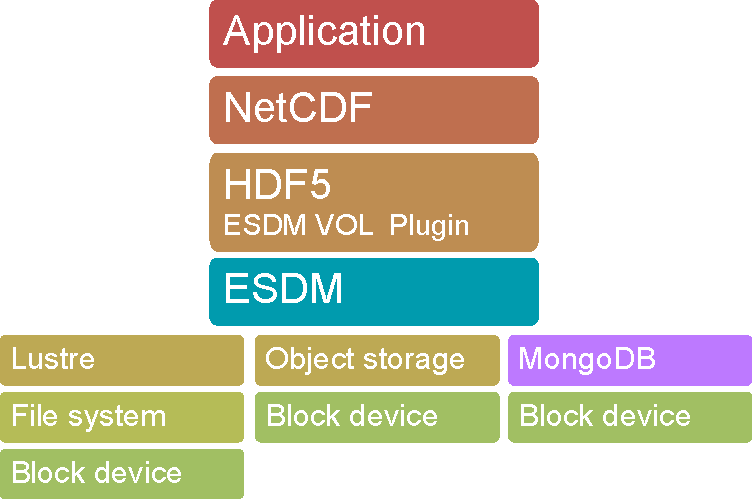
\includegraphics[width=0.5\columnwidth]{figures/layers-esdm}
	\caption{A typical I/O-stack with the ESD middleware}
	\label{fig:architecture-esd-layering}
\end{figure}

\begin{figure}[bp]
	\centering
	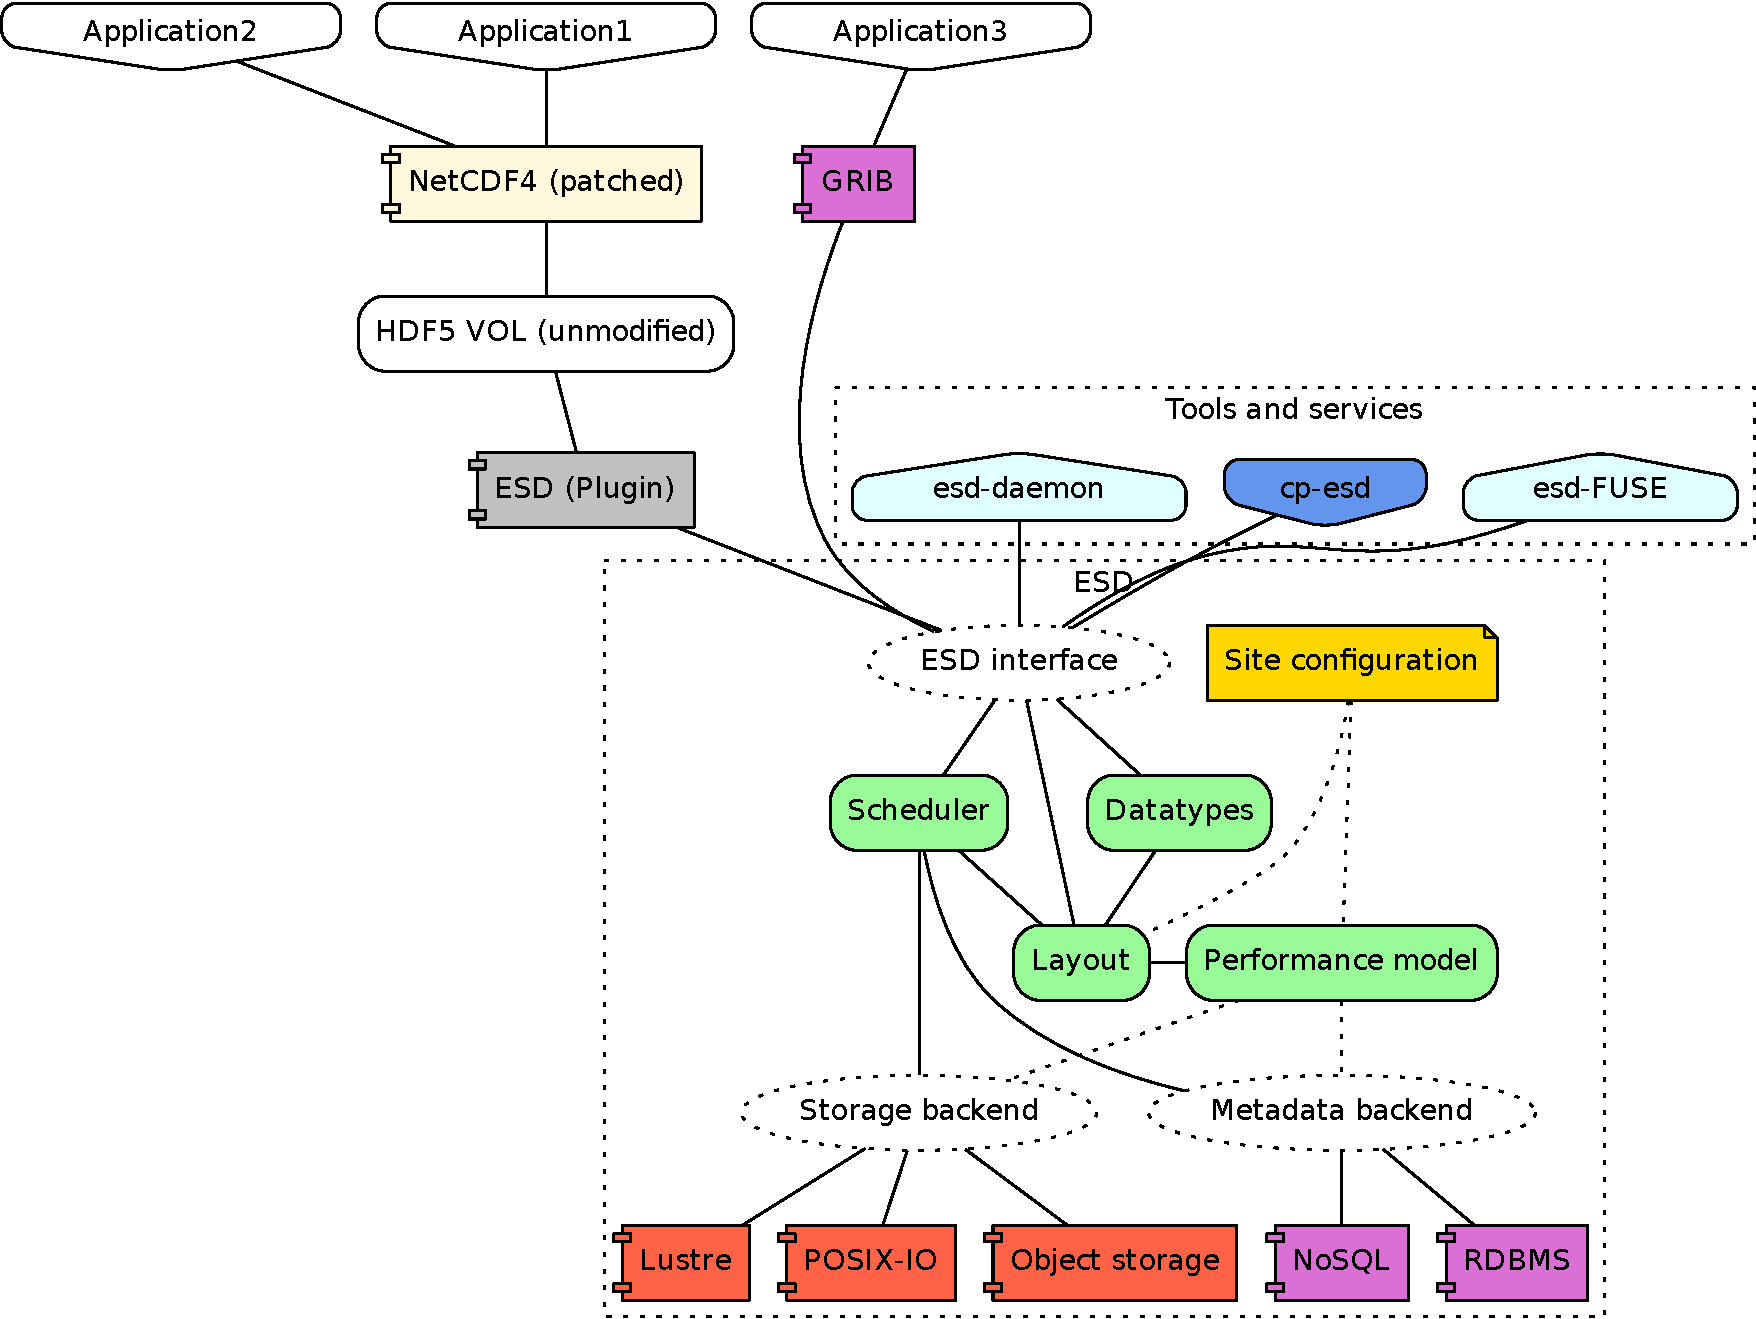
\includegraphics[width=0.98\columnwidth]{architecture-backend_with-scheduler/architecture-backend-src.pdf}
	\caption{Overview of the ESD architecture, relevant components and relationship to application and storage systems.}
	\label{fig:architecture}
\end{figure}

A typical I/O-stack for an application using ESDM is shown in \Cref{fig:architecture-esd-layering}.
I/O of an existing application using the NetCDF (or HDF5) interface is processed by the ESDM plugin of HDF5 which may decide to store data on one of the available
storage backends such as Lustre or an Object storage.
Metadata may be stored in one of the supported metadata plugins.
The user does not have to make decisions regarding the storage or metadata backends to be used; this decision is made by the middleware.

\bigskip


Details of the ESDM architecture is given in \Cref{fig:architecture}.
It provides more details about how ESDM is embedded into the existing software landscape and its high-level components:

\paragraph{Applications}
Use existing storage interfaces such as NetCDF4, GRIB or they may use the ESD interface.

\paragraph{Job scheduler}
The job scheduler assigns supercomputer resources to jobs.
It may use the ESD interface to inform about future activity and stage/unstage data.


\paragraph{Middleware libraries} are adjusted to be layered on top of the ESD interface.


%%%%%%%%%%%%%%%%%%%%%%%%%%%%%%%%%%%%%%%%%%%%%%%%%%%%%%%%%%%%%%%%%%%%%%%%%%%%%%%
\paragraph{ESD Interface}
This represents the API exposed to other libraries and users.
The API is independent of the specific I/O backend used to store the data and supports structured queries to perform complex data selections in the variables.
The API is able to support the complex workflows of future applications.

%%%%%%%%%%%%%%%%%%%%%%%%%%%%%%%%%%%%%%%%%%%%%%%%%%%%%%%%%%%%%%%%%%%%%%%%%%%%%%%
\paragraph{Data Types}
The datatype component provides native data types that can be used by users or other libraries to describe data points inside variables.
We follow the approach pursued by the MPI and HDF5 libraries, that is, we provide a set of native data types and a basic set of datatype constructors that can be used to build custom derived datatypes.

%%%%%%%%%%%%%%%%%%%%%%%%%%%%%%%%%%%%%%%%%%%%%%%%%%%%%%%%%%%%%%%%%%%%%%%%%%%%%%%
\paragraph{Layout}
The layout component allows the middleware to store pieces of data on different backends depending on specific site configuration contained in the performance model.
The layout component in this case takes responsibility for generating additional technical metadata describing data placement and for storing it in the appropriate metadata backend (i.e. MongoDB).
A more detailed description of what technical metadata is, is given in the rest of this section.

\paragraph{Performance model}
This model predicts performance for data access using a site-specific configuration that describes the characteristics of available hardware technology.
It is used by the layout component to make decisions of the data placement.

\paragraph{Scheduler}
The scheduler queues asynchronous calls from the API and processes them.
It dispatches calls to storage and metadata backends and uses the layout component to identify beneficial placement of data.

\paragraph{Metadata backend}
Responsible to store all technical and scientific relevant metadata providing efficient access and manipulation.

\paragraph{Storage backend}
These backends are responsible to transform ESD objects and data structures to storage-technology-specific representations.


\paragraph{Tools and services}
On top of ESDM several user space tools are provided, a few examples are:
The FUSE client provides backwards POSIX compatibility with existing applications.
The daemon checks the consistency and integrity of the data managed by ESDM, potentially triggering actions to clean up and replicate data.
The copy tool allows importing and exporting data from ESD to an existing storage infrastructure.
It also serves as blue-print to embed its capabilities into higher-level tools such as GridFTP.



%%%%%%%%%%%%%%%%%%%%%%%%%%%%%%%%%%%%%%%%%%%%%
%\subsection{Component Responsibilities}
%\label{sec: viewpoints/logical/responsibilities}


%%%%%%%%%%%%%%%%%%%%%%%%%%%%%%%%%%%%%%%%%%%%%%%%%%%%%%%%%%%%%%%%%%%%%%%%%%%%%%%%%%%%%%%%%%
\section{Logical View: Data Model}
\label{sec: viewpoints/logical/data model}


While data types introduced by computer architectures and software libraries are important for the data model, they are discussed separately in \Cref{sec: viewpoints/logical/datatypes}.



The data model of a system organises elements of data, standardises how they represent data entities and how users can interact with the data.
The model can be split into three layers:
\begin{enumerate}
	\item The \textbf{conceptual data model} describes the entities and the semantics of the domain that are represented by the data model and the typical operations to manipulate the data.
	In our case, the scientific domain is NWP/climate.
	\item The \textbf{logical data model} describes the abstraction level provided by the system, how domain entities are mapped to objects provided by the system\footnote{A entity of the domain model such as a car could be mapped to one or several objects.}, and the supported operations to access and manipulate these objects are defined.
	Importantly, the \textbf{logical data model} defines the semantics when using the operations to access and manipulate the system objects.
	For example, a system object of a relational model is a table -- representing attributes of a set of objects -- and a row of a table representing attributes of a single object.
	\item The physical data model describes how the logical entities are finally mapped to objects/files/regions on available hardware.
	The physical data model is partly covered by the backends of ESDM, therefore, the descriptions will stop at that abstraction level.
\end{enumerate}

\subsection{Conceptual Data Model}
\label{subsec: conceptual data model}

Our conceptual data model is aligned with the needs of domain scientists from climate and weather. It reuses and extends from concepts introduced in a data model proposed for the Climate and Forecasting conventions for NetCDF data\footnote {\url{``A CF Data Model and Implementation'', Hassel et al, 2017, GMD submitted}}.

\paragraph{Motivation from climate}



The ESDM needs to store, identify and manipulate data variables,  $V$, containing scientific data from the (continuous) real or model world, discretised within a ``sampling'' domain $d$, that is
\[V=V(d)\]
where $V$ may be air temperature, for instance. The domain $d$ describes the location for each value of $V$, and is a function of its independent dimensions, for instance
\[d = d(Z(z), Y(y), X(x)))\]
where $d$ is a three-dimensional domain described by axes of height, latitude, and longitude, sampled at coordinates found from the complete set of samples $Z(z),Y(y),X(x)$.
Each set of coordinates $x,y,z$  together specifies a location in the atmosphere at which $V$ is specified.



The full dimensionality of the variable may exceed the number of dimensions needed to store it --- for example, if $V$ is air-temperature at 1.5m, then $V$ may be sampled (and stored) in multiple 2-dimensional $x,y$ arrays, with each additional array representing a different time step.
In this case, some extra dimensions may be stored in metadata accompanying the scientific data.



Sampling may be regularly spaced along one or more of the dimensions, in which case the coordinates (e.g., $x$) of the samples can be found algorithmically from the dimensions (e.g., $X$), and we describe the coordinate-grid as ``structured'' in those dimensions; but they can also be irregularly spaced, and their individual positions may need to be stored, in which case we describe the grid as ``unstructured'' in those dimensions.
With an unstructured grid it is not possible to fully understand the domain distribution of $V$ unless all the coordinates are themselves stored as variables (e.g., $Z(z)$ is itself a variable defined at coordinates over a 1-dimensional domain spanning the height dimension).  A coordinate grid may be structured in one set of dimensions and unstructured in another.

\paragraph{}The values of $V$ at the coordinate positions may represent a value at that point, or be representative of an area, volume or face of a cell defined in one or more of the dimensions.

\paragraph{}In summary then, the conceptual (or scientific) data model consists of the following key entities:

\paragraph {Variable:} A variable, $V$, defines a set of data representing a discrete (generally scalar) quantity discretised within a ``sampling'' domain, $d$.  It is accompanied by

\paragraph {Metadata:} which will include at the minimum, a name, but may also include units, and information about additional dimensionality, directly (e.g. via a key, value pair such as that necessary to expose $z=1.5m$ for air temperature at 1.5m) or indirectly (e.g. via pointers to other generic coordinate variables which describe the sampled domain).   There may also be a dictionary of additional metadata which may or may not conform to an external semantic convention or standard.  Such metadata could include information about the tool used to observe or simulate the specific variable.  Additional metadata is also required for all the other entities described below.

\paragraph{Dimension:} The sampling domain $d$ is defined by Dimensions which also defines coordinate axis. Dimensions will include metadata, which have to include at a minimum a name (e.g. height, time), but may also include information about directionality, units (e.g. degrees, months, days-since-a-particular-time-using-a-particular-calendar), or details of how to construct an algorithm to find the actual sampling coordinates, perhaps using a well-known algorithm such as an ISO 8601 time.

\paragraph{Coordinate:} Coordinates  are the set of values at which data is sampled along any given dimension. They may be
explicitly defined by indexing into a coordinate variable, or implicitly defined by an algorithm. When we talk about the coordinates, it is usually clear if we mean the N-dimensional coordinate to address data in a given variable or if we just mean the (1D) coordinate along one dimension.


\paragraph{Cell:} The data values are known at points, which may or may not represent a cell. Such cells are N-dimensional shapes where the dimensionality may or may not fully encompass the dimensionality of the domain.
N-dimensional shapes can be implicitly defined in which case the Cartesian product of all dimensional coordinates forms the data "cube" of the cell, but they can also be explicitly defined, either by providing bounds on the coordinate variables (via metadata) or by introducing a new variable which explicitly defines the functional boundaries of the cell (as might happen in a finite element unstructured grid).


\paragraph{Data set:} Variables can be aggregated into data sets. A data set contains multiple variables that logically belong together, and should be associated with metadata describing the reason for the aggregation.  Variables must have unique names within a data set.



Our conceptual model assumes that all variables are scalars, but clearly to make use of these scalars requires more complex interpretation.
% In particular, we need to know the... ??? TODO

\paragraph{Datatype:}
which defines the types of values that are valid and the operations that can be conducted.
While we are mostly dealing with scalars, they may not be amenable to interpretation as simple numbers.
For example, a variable may be storing an integer which points into a taxonomy of categories of land-surface-types.
More complex structures could include complex data types such as vectors, compressed ensemble values, or structures within this system, provided such interpretation is handled outside of the ESDM, and documented in metadata.  This allows us to limit ourselves to simple data types plus arbitrary length blocks of bits.

\paragraph{Operators:} Define the manipulations possible on the conceptual entities. The simplest operators will include creation, read, update and delete applied to an entity as a whole, or to a subset, however even these simple operators will come with constraints, for example, it should not  be possible to delete a coordinate variable without deleting the parent variable as well. There will need to be a separation of concerns between operators which can be handled  \textit{within} the ESDM subsystem, and those which require external logic. Operators which might require external logic include subsetting --- it will be seen that the ESDM will support simple subsetting using simple coordinates ---  but complex subsets such as finding a region in real space from dimensions spanned using an algorithm or coordinate variable, may require knowledge of how such algorithms or variables are specified.
Such knowledge is embedded in conventions such as the CF NetCDF conventions, and this knowledge could only be provided to the ESDM via appropriate operator plugins.

%\begin{figure}[b]
%	\centering
%	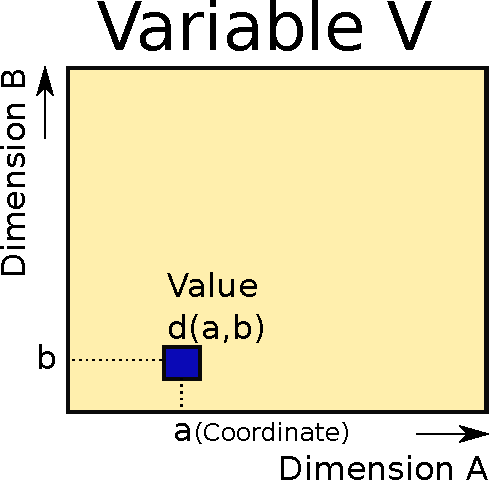
\includegraphics[width=5cm]{figures/data-model-variable}
%	\caption{Illustration of a 2D variable}
%	\label{fig:domainEntities}
%\end{figure}
% If we really want a figure, I've got a better one (BNL)



Whatever the sampling regime and dimensionality, values of of a variable $V$ will be laid out in storage. In the next section (\ref{subsec-ldm}) we present the logical data model associated with the storage, before presenting a mapping of the conceptual data model to storage in section \ref{subsec-mapping}).


\subsection{Logical Data Model}
\label {subsec-ldm}

The logical data model describes how data is represented inside ESDM, the operations to interact with the data and their semantics. There are four first class entities in the ESDM logical data model: \textbf{variable}s, \textbf{fragment}s, \textbf{container}s, and \textbf{metadata}. ESDM entities may be linked by ESDM \textbf{reference}s, and a key property which emerges from the use of references is that no ESDM entity instance may be deleted while references to it still exist. The use of reference counting will ensure this property as well as avoid dangling pointers.

\Cref{fig:data-model} gives an overview of the logical data model.



Each of these entities is now described, along with a list of supported operations:

\paragraph{Variable:} In the logical data model, the variable corresponds directly to a variable in the conceptual data model. Each element of the variable sampled across the dimensions contains data with a prescribed \textbf{DataType}.
Variables are associated with both \textbf{Scientific Metadata} and \textbf{Technical Metadata}. Variables are partitioned into \textbf{fragments} each of which can be stored on one or more ``storage backend''.
A variable definition includes internal information about the domain (bounding box in some coordinate system)  and dimensionality (size and shape), while the detailed information about which coordinate variables are needed to span the dimensions and how they are defined is held in the technical metadata.  Similarly, where a variable is itself a coordinate variable, a link to the parent variable for which it is used is held in the technical metadata.
The ESDM will not allow an attempt to delete a variable to succeed while any such references exist (see references).
A key part of the variable definition is the list of fragments associated with it, and if possible, how they are organised to span the domain.
Users may choose to submit code pieces that are then run within the I/O-path (not part within ESiWACE implementation), such an operation covers the typical filter, map and reduce operations of the data flow programming paradigm.

Fragments are created by the backend while appending/modifying data to a variable.

\textbf{Operations:}
\begin{itemize}
	\item Variables can be created and deleted.
	\item Fragments of data can be attached and deleted.
	\item Fragments can be repartitioned and reshuffled.
	\item Integrity can be checked.
	\item Data can be read, appended or modified those operations will be translated to the responsible fragments.
	\item Metadata can be atomically attached to a variable or modified.
	\item A variable can be sealed to make it immutable for all subsequent modifications.
	\item Process data of the variable somewhere in the I/O-path.
\end{itemize}

\paragraph{Fragment:}  A fragment is a piece (subdomain) of a variable. The ESDM expects to handle fragments as atomic entities, that is, only one process can write  a fragment through the ESDM, and the ESDM will write fragments as atomic entities to storage backends.
The backends are free to further partition these fragments as is appropriate, for example, by sharding using chunks as described in section \ref{subsec-mapping}.
However, the ESDM is free to replicate fragments or subsets of fragments and to choose which backend is appropriate for any given fragment.
This allows, for example, the ESDM to split a variable into fragments some of which are on stored on a parallel file system, while others are placed in object storage.

\textbf{Operations:}
\begin{itemize}
	\item Data of fragments can be read, appended or modified.
	\item Integrity of the fragment can be checked.
	\item Process data of the variable somewhere in the I/O-path.
\end{itemize}
%\todo{Resolve question on slack: \url{https://esiwace.slack.com/archives/C2T7KDRGC/p1496396797771552}}

\paragraph{Container:} A container is a virtual entity providing views on collections of variables, allowing multiple different data sets (as defined in the conceptual model) to be realised over the variables visible to the ESDM.  Each container provides a hierarchical namespace holding references to one or multiple variables together with metadata.Variables cannot be deleted while they are referenced by a container.  The use of these dynamic containers provides support for much more flexible organisation of data than provided by a regular file system semantics --- and efficiently support high level applications such as the Data Reference Syntax\footnote{Taylor et al (2012): CMIP5 Data Reference Syntax (DRS) and
Controlled Vocabularies.}.

A container provides the ESDM storage abstraction which is analogous to an external file. Because many scientific metadata conventions are based on semantic structures which span variables within a file in ways that may be opaque to the ESDM without the use of a plugin, the use of a container can indicate to the ESDM that these variables are linked even though the ESDM does not understand why, and so they cannot be independently deleted.
When entire files in NetCDF format are ingested into the ESDM, the respective importing tool must create  a container to ensure such linking properties are not lost.

\textbf{Operations:}
\begin{itemize}
	\item Creation and deletion of containers.
	\item Creation and deletion of names in the hierarchical name space; the creation of links to an existing variable.
	\item Attaching and modification of metadata.
	\item Integrity can be checked.
\end{itemize}

\paragraph{Metadata:} can be associated with all the other first class entities (variables, fragments, and containers). Such metadata is split into internal ESDM technical metadata, and external user-supplied semantic metadata.
%A future version of the ESDM will support the internal exploitation of external metadata via plugins, but this version of the ESDM will treat external metadata as atomic and opaque, and simply serialise and store/replace/delete any such metadata. The internal metadata ...
%\todo {There needs to be a formal description of internal metadata}
Technical metadata covers, for example, permissions, information about data location and timestamps.
A backend will be able to add its own metadata to provide the information to lookup the data for the fragment from the storage backend managed by it.
Metadata by itself is treated like a normal ESDM variable but linked to the variable of choice.
The implementation may embed (simple) metadata into fragments of original data (see Reference).

\textbf{Operations:}
\begin{itemize}
	\item Uses can create, read, or delete arbitrary scientific metadata onto variables and containers.
	A future version of the ESDM may support user scientific metadata for fragments.
	\item Container level metadata is generally not directly associated with variables, but may be retrieved via following
	references from variables to containers.
	\item Queries allow to search for arbitrary metadata, e.g., for objects that have (\texttt{experiment=X, model=Y, time=yesterday}) returning the variables and containers in a list that match.
	This enables to locate scientific data in an arbitrary namespace.
\end{itemize}

\paragraph{Reference}
A reference is a link between entities and can be used in many places, references can be embedded instead of real data of these logical objects.
For example, dimensions inside a variable can be references, also a container typically uses references to variables.

\textbf{Operations:}
\begin{itemize}
	\item A reference can be created from existing logical entities or removed.
\end{itemize}


%\paragraph{Set}
%A set contains objects but only one object.




\begin{figure}
	\centering
	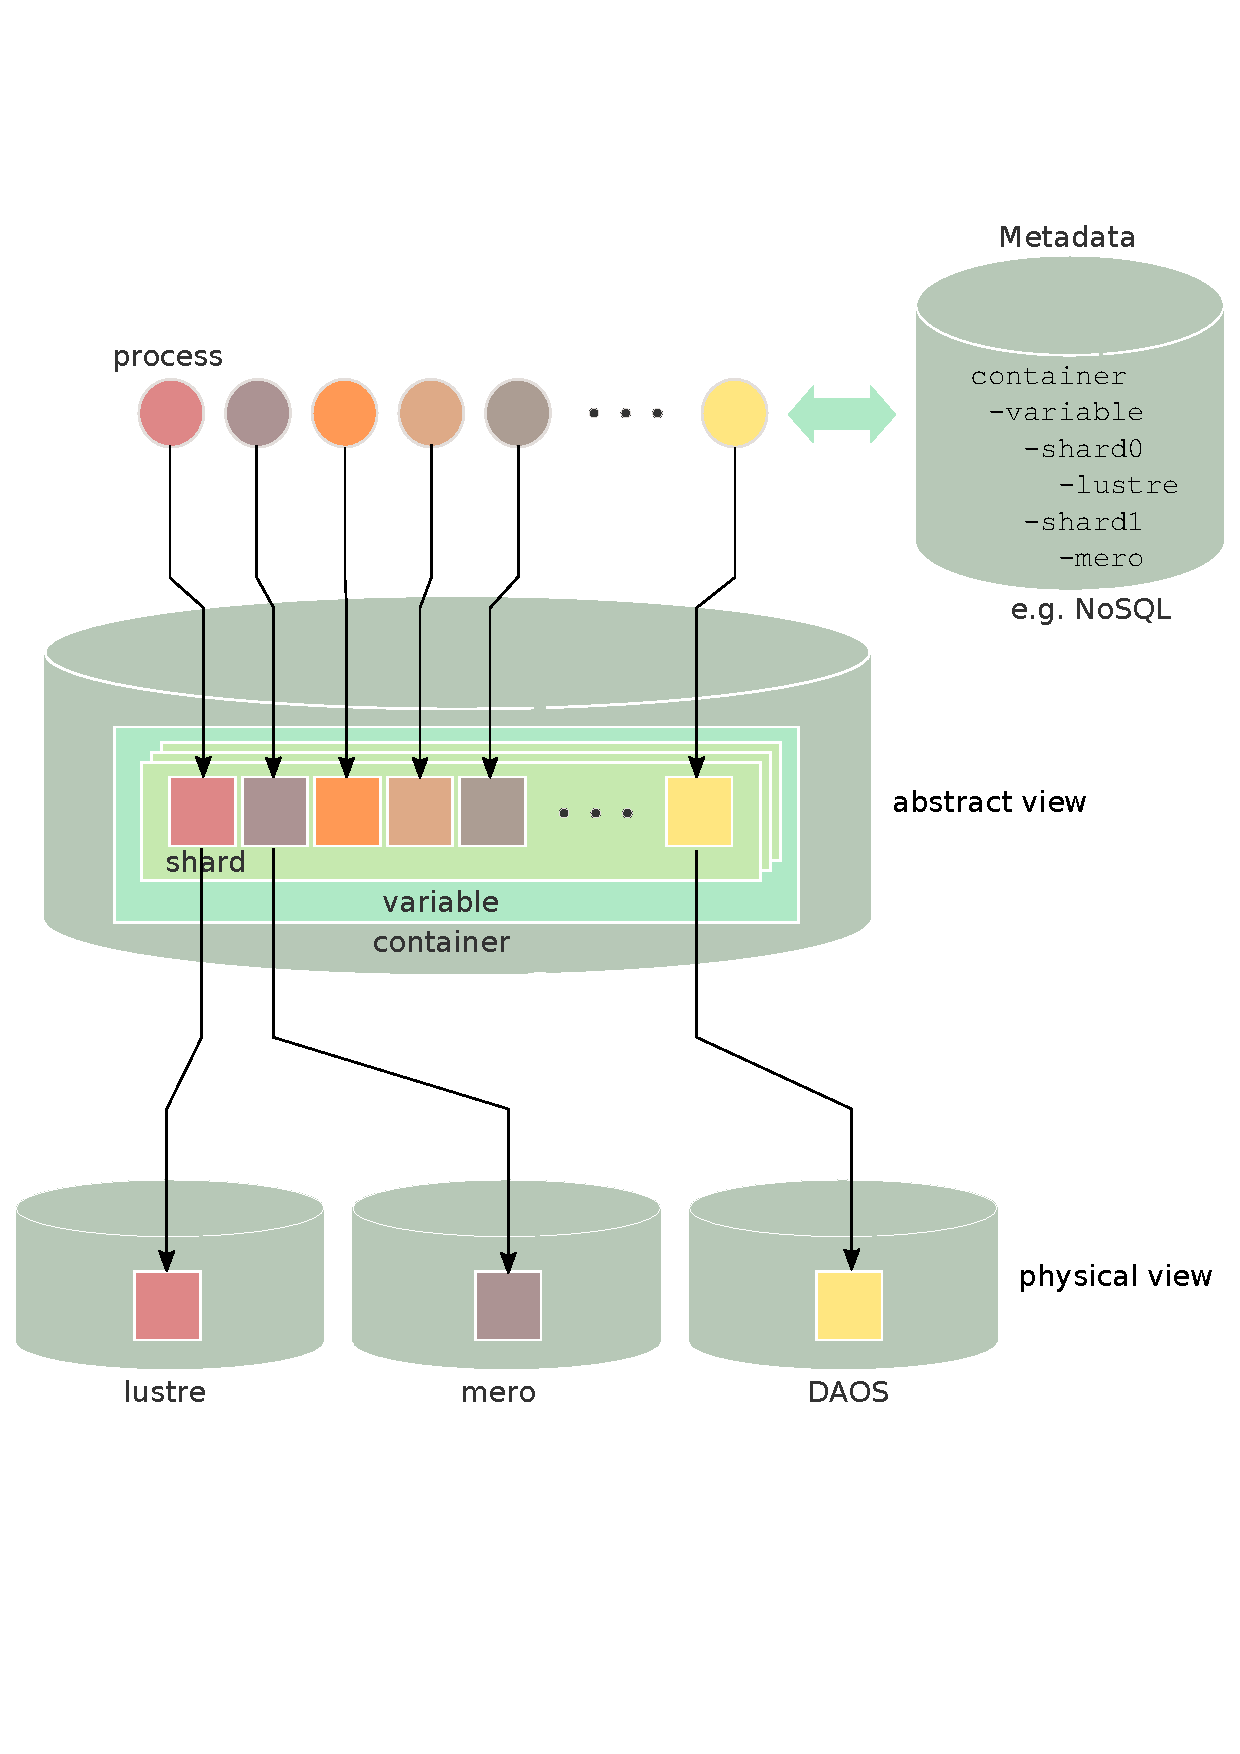
\includegraphics[width=0.5\textwidth]{data-model}
	\caption{Logical Data Model}
	\label{fig:data-model}
\end{figure}

\paragraph{Namespace}

ESDM does not offer a simple hierarchical namespace for the files.
It provides the elementary functions to navigate data: teleportation and orientation in the following fashion:
Queries about semantical data properties (e.g., \texttt{experiment=myExperiment, model=myModel, date=yesterday}) can be performed returning a list of matching files with their respective metadata.
Iterating the list (orientation) is similar to listing a directory in a file system.

Note that this reduces the burden to define a hierarchical namespace and for data sharing services based on scientific metadata.
An input/output container for an application can be assembled on the fly by using queries and name the resulting entities.
As a container provides a hierarchical namespace,
by harnessing this capability one can search for relevant variables and map them into the local file system tree, accessing these variables as if they would be, for example, NetCDF files.
By offering a FUSE client, this feature also enables backwards compatibility for legacy POSIX applications.



\subsection{Relationships between the Conceptual and Logical Data Model}
\label{subsec-mapping}

The conceptual data model and logical data model are described above, and summarised in \Cref{fig:cdm_ldm}.
These UML and this version of the architecture do not fully deal with the issues around coordinate systems which are not described by simple monotonic coordinate arrays, for which simple bounding boxes can be constructed.

As noted above, to fully exploit more complicated coordinate systems it will be necessary to describe those coordinate systems more fully in the scientific metadata (LDM\_Sci\_Metadata) and potentially provide a plugin to the system to handle them.
This notion is shown in the UML by virtue of the optional use of a named plugin to be identified in the scientific metadata, but the details of how that will work has been postponed to the prototype development.

\begin{figure}
	\centering
	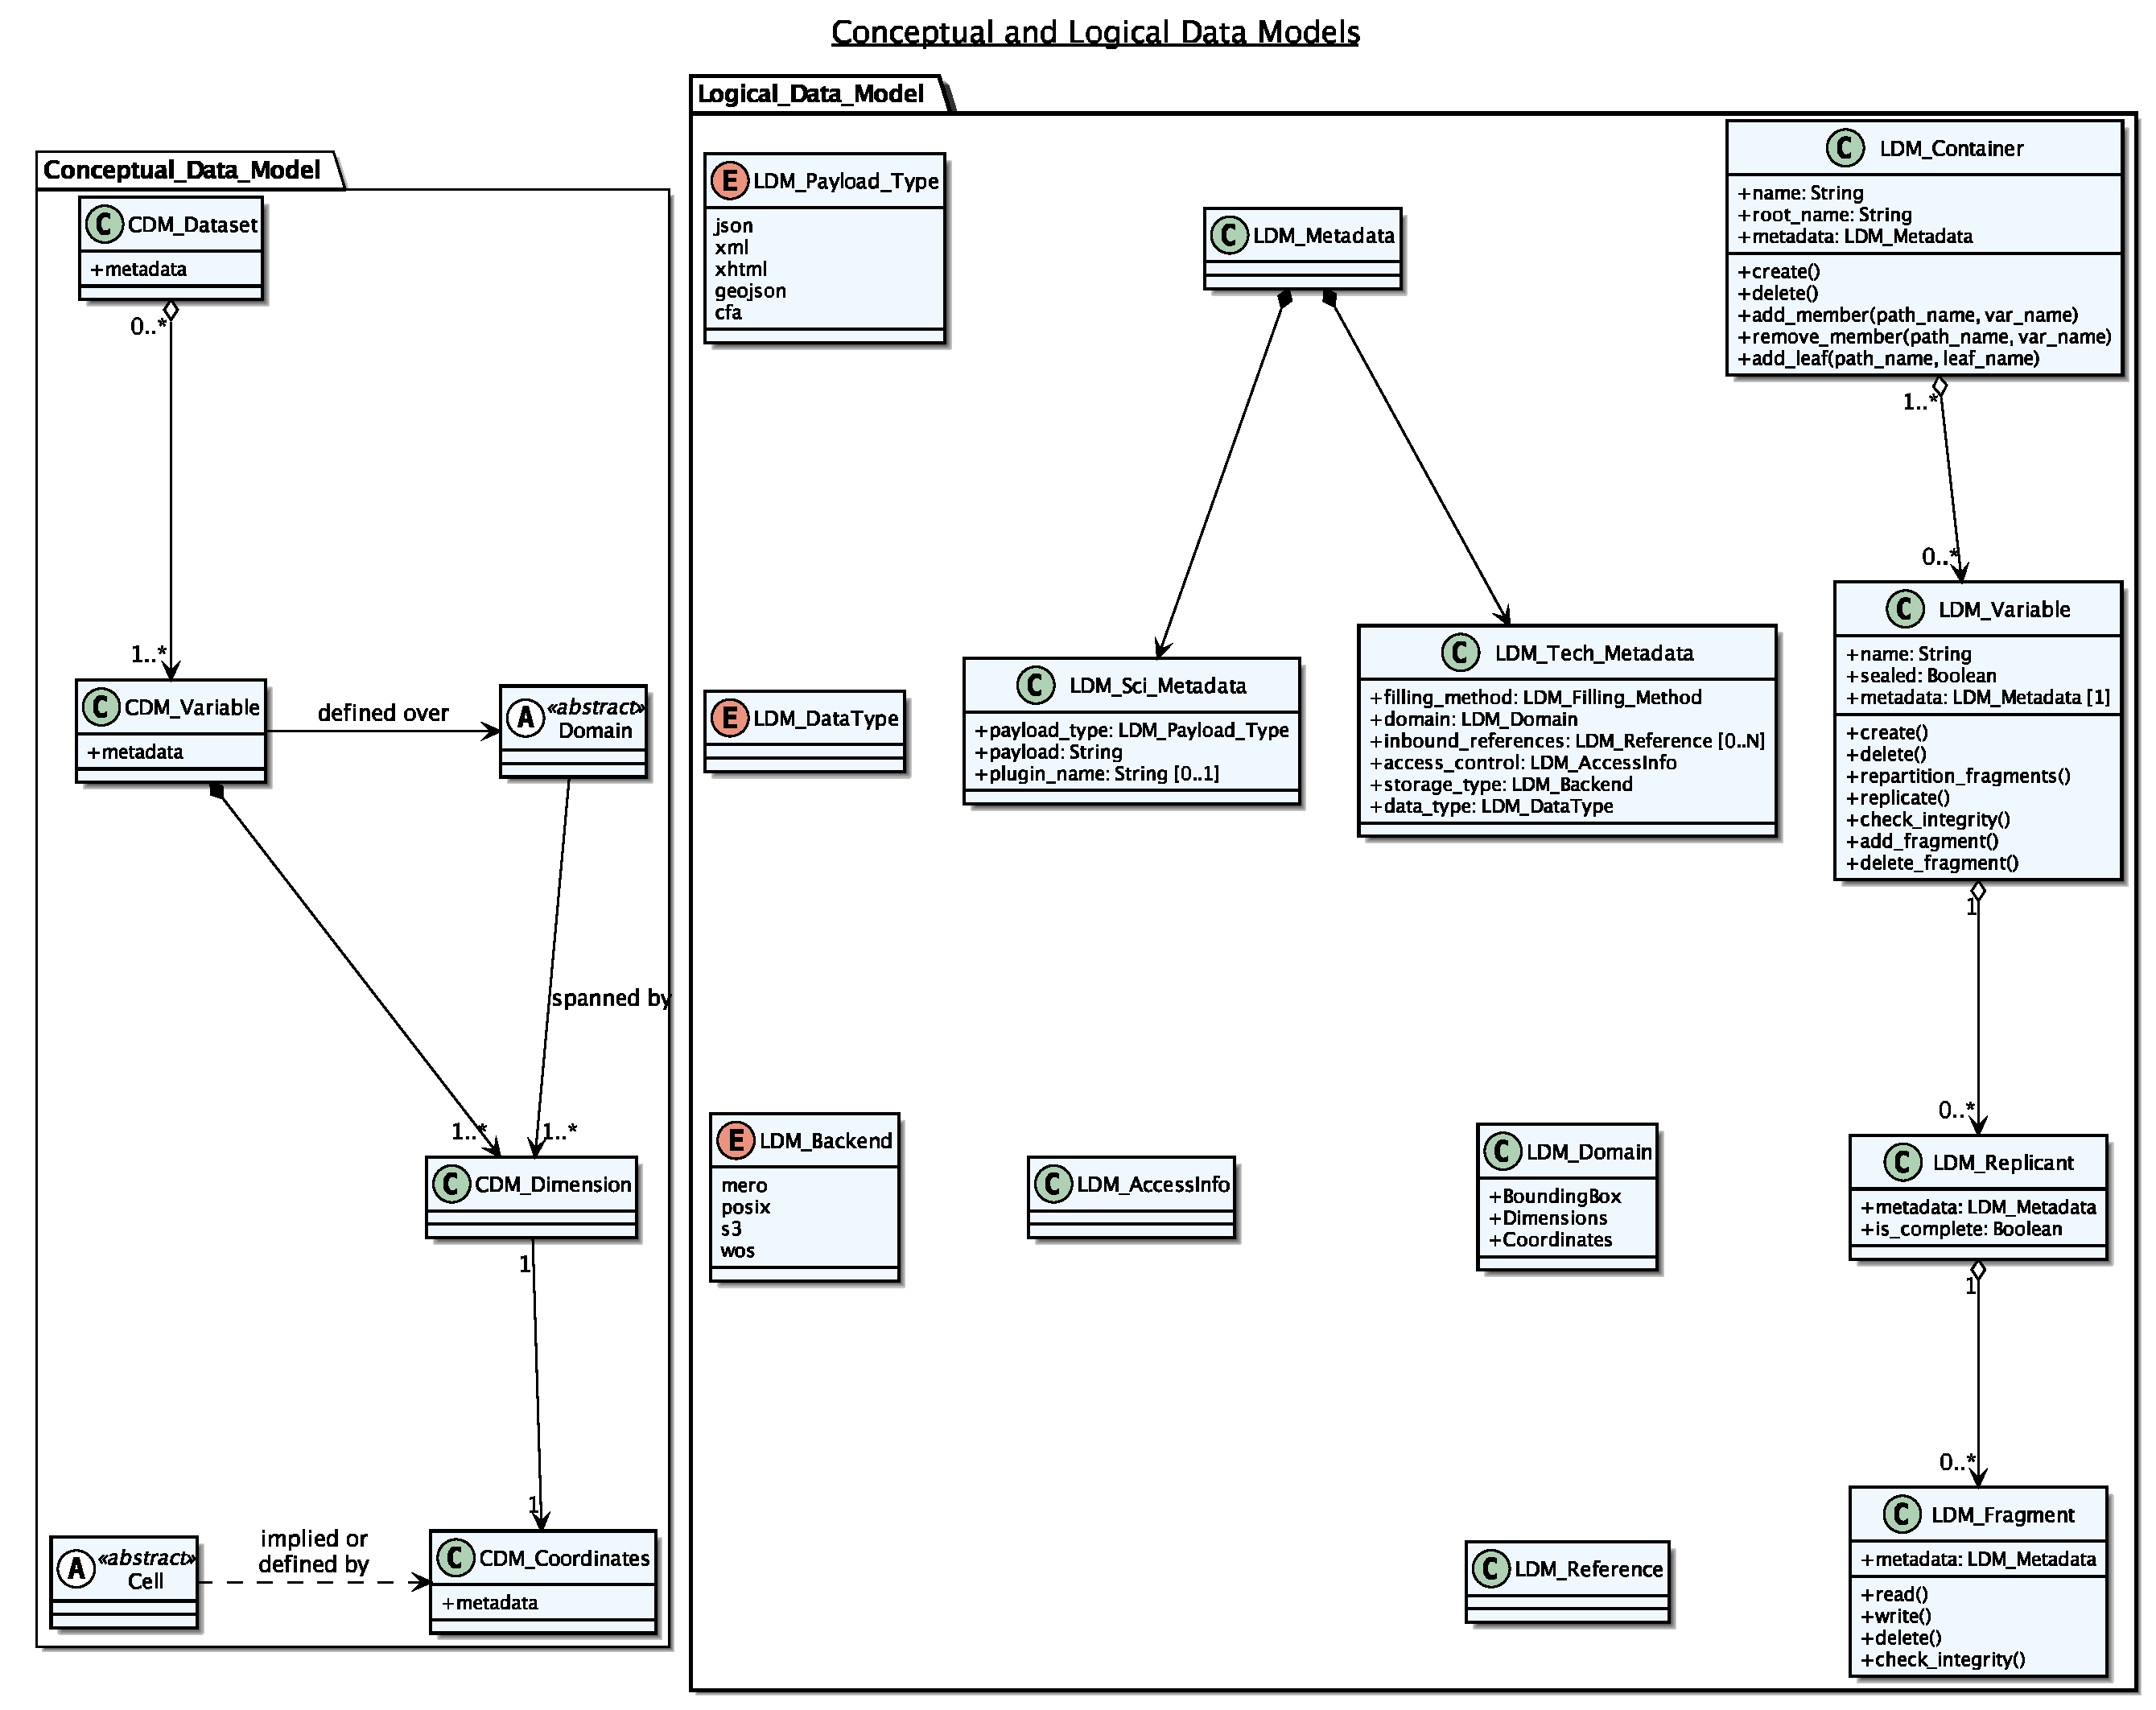
\includegraphics[width=\textwidth]{inf-model/cdm_ldm.eps}
	\caption{A non-normative UML version of the conceptual and logical data models.
	The figure includes example for the operators of the individual logical operations.
	These UML are expected to be updated as the system is developed.  See also figure \ref{fig:dm_map}.}
	\label{fig:cdm_ldm}
\end{figure}

The key high level entities are the conceptual container, variable, and domain, which have direct correspondence in the logical
data model (see \Cref{fig:dm_map}) --- however it is important to recognise that these are not isomorphic relationships. For example,
the concept of a domain of a variable in the conceptual model is expanded in the logical data model to include sub-domains associated
with fragments, but the same class is used for both usages (LDM\_Domain for both variable domain and fragment sub-domain).

\begin{figure}
	\centering
	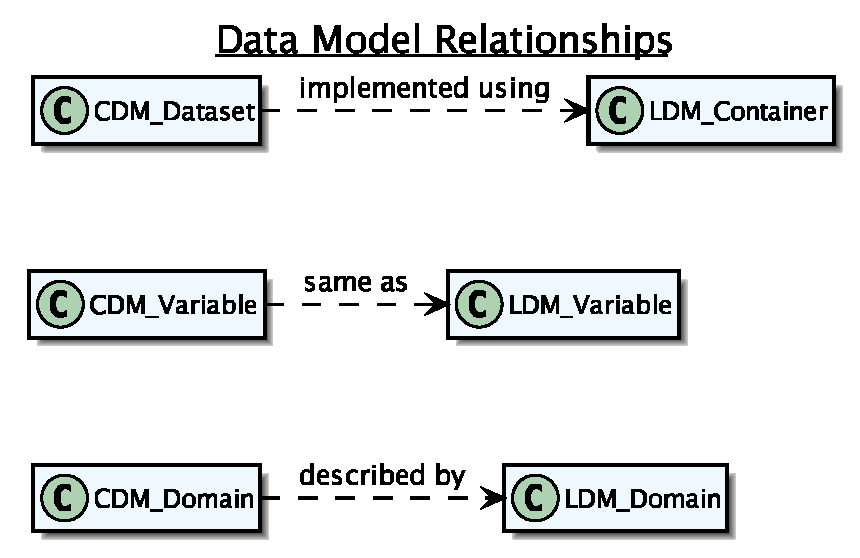
\includegraphics[scale=0.6]{inf-model/cdm_cdm.eps}
	\caption{Key relationships between conceptual and logical data models.}
	\label{fig:dm_map}
\end{figure}


%\subsection{Metadata mapping: Needs updating}
%\todo{Some examples driven from the use cases}
%

%%%%%%%%%%%%%%%%%%%%%%%%%%%%%%%%%%%%%%%%%%%%%%%%%%%%%%%%%%%%%%%%%%%%%%%%%%%%%%%
\subsubsection{Adaptive Data Mappings}
The typical storage mapping for scientific data format libraries is the file (linear sequence of bytes organized following the POSIX file system representation, i.e. inodes and blocks). Information is translated into a linear array of bytes in the file system using appropriate schemas. Since the data model defined by the data format library can contain complex hierarchies and attributes besides raw data, the final file will contain additional scientific metadata that needs to be accessed using the POSIX-IO data interface (e.g. \texttt{read()} and \texttt{write()}) instead of the file metadata interface (e.g. \texttt{stat()}, \texttt{lookup()}). This makes the storage model adopted by data format libraries incompatible with the typical parallel file system organization, in which metadata and data are splitted apart and assigned to different services for optimal performance. Additionally, new storage system paradigms have emerged in the last years in which files are organized in a flat namespace (e.g. object storage), removing the restrictions imposed by metadata operations like namespace traversal of POSIX file systems. Hierarchical organization can be still achieved using other dedicated storage representations like key-value stores, at the expense of reduced POSIX semantic.

There is therefore a necessity for more flexible data mappings that can take advantage of an increasing number of storage and backend alternatives, improving access efficiency at the same time. There are two different approaches to this problem: the first is to develop a new data mapping schema for every storage backend. This is the solution adopted by the HDF5 library (through the virtual file and the virtual object layers) in which multiple storage backends can be employed by developing a corresponding plugin that contains the right mapping schema. The obvious limitation of this solution is that once the user has selected a certain backend for a file, this cannot be changed without migrating the whole file to another backend. The second approach is more flexible and consists in making the storage backend selection adaptive. This has the advantage of enabling backend storage selection on the fly depending upon the type of data being stored or a set of user/system defined parameters (e.g. list of data placement policies satisfying certain requirements of quality of service).

Our proposed solution is to integrate the adaptive data mappings capabilities just discussed in the layout component of the ESD middleware. The middleware will understand the scientific metadata of other relevant data format libraries and will be able to use multiple storage backends at the same time to store and retrieve different pieces of data. To support multiple formats the datatype component in the ESD middleware will expose a datatype interface similar to the one available in HDF5 (described in Section~\ref{sec: data-formats}). Additionally, the middleware will add significant metadata to be used in the life cycle management and sharing of data. This can include semantic metadata describing which data is needed and how it is going to be used, the required level of resilience, etc. In this context, some metadata can be automatically generated by the middleware or defined by the user and passed to the middleware through an apposite interface (that will be part of the ESD exposed interface).

Legacy codes will have access to data using a familiar POSIX interface exported through an ESD FUSE module. The FUSE module will communicate with the ESD middleware to access data and export it to users using a namespace representation. The mapping schema definition for mapping data between the storage representation and the namespace will be done later in the project.

Another important aspect to consider when talking about adaptive data mappings is the storage tiering, that is, how many levels of storage there are in the system. Historically, HPC applications have relied on parallel file systems as first tier to store and retrieve their data. Besides the parallel file system, most high-end clusters have a second level of archival storage to which data is migrated from the parallel file system using a hierarchical storage manager. Nowadays compute nodes have access to local storage (typically a block device formatted with a local file system) and with the emergence of new storage technologies, such as non-volatile memories, permanent byte addressable memory. The ESD middleware should be able to exploit these local storage resources to implement prefetching strategies (read patterns) and burst buffers (write patterns).

%In the specific case of Mero (Seagate object store system), which represents one of the possible storage backends that has to be supported by the ESD middleware, hierarchical and semantic metadata can be stored in the key-value store service while array data can be stored into objects. In fact, we can think about using more than one object per dataset. This is particularly useful with chunking since every chunk in the dataset can be mapped to a different object, making parallel access to different data units possible without any need for I/O coordination (no false sharing is possible in this case). Of course, I/O coordination still needs to be provided when multiple processes access the same dataset and chunking is not enabled. In this case the ROMIO library already provides a collective I/O implementation that can be reused by the ESD middleware. Whenever needed, false sharing of data can also be avoided by using `persistent file realm' like mechanisms\footnote{This mechanism allows a certain file portion to be assigned to a specific process in the application and makes this assignment persistent across multiple data accesses.}.

%\todo{Giuseppe: you had a very good document on this already can add something here}

%Goal of the dynamic mapping is to create a hierarchical namespace based on the available metadata.
%It is based on the search for objects.
%With the help of FUSE, these mappings can be created based on a user configuration upon mount-time (supports user mounts).
%Inaccessible data, i.e., where the permissions are not sufficient, can be hidden from the namespace.

%An example mapping could be:
%“v.info.model/v.info.environment.date/v.info.experiment.tags/v.info.name <as NC4>”.
%This would show a single NetCDF4 file for each variable.
%If a variable is attached to various tags, then it is shown for each of them.

%“v.info.model/v.info.environment.date/v.domain.time/v.info.name <as NC4>”.
%Would show one file per timestep.

%How to resolve ambiguity?

%Existing containers can also be directly mapped, showing the input and output variables similarly:
%“<c.\_id>/<c.directory>”


%The storage should now how the logical data space maps to physical positions in memory or storage.
%If the storage backends have this knowlege, they can run local operations on the data.

%Alternatives:
%Triangular grid (locally refined), somehow mapped from user-space to a 1D structure which gets mapped to the storage. (Traditional approach)

%Application(data structure) - Mapping - Middleware - Mapping (byte array) - Storage API - Storage backend

%or:

%Application - Middleware - Storage API - Mapping - Storage backend

%Use sth. like MPI datatypes to descripe memory (in the application)
%Add metadata to describe the meaning / semantics, additional gain: resilience because we know which data to replicate to put into triple ECC ...
%Add hints how the data is used / will the used in the future

%Avoid redundant descriptions of memory / storage.
%Users stores a 3D field, it is clear which storage location is responsible for [x,y,z]
%How to store triangles etc.

%Why not store code as description?
%- describes neighborhood?

%Coordinates? Universal coordinates, application coordinates?

%VTK? haben diverse Datenstrukturen hierfÃŒr.


%Separation of concerns...

%Missmatch of Chunks size and application domain

%false sharing

%Pointer Datentyp: strong ptr, weak ptr.
%like Boost usw.


%NVRAM



%%%%%%%%%%%%%%%%%%%%%%%%%%%%%%%%%%%%%%%%%%%%%%%%%%%%%%%%%%%%%%%%%%%%%%%%%%%%%%%
\subsubsection{Technical Metadata}
\label{subsec: technical metadata}

Besides scientific metadata, the dynamic mapping of data to storage backends requires further metadata that must be managed.
To distinguish technical metadata from scientific metadata, an internal namespace is created.
Relevant metadata is shown in \Cref{tbl:additionalTechnicalMetadata} for shards, variables and containers, respectively.

Metadata can be optional (O) or mandatory (M), and either is created automatically or must be set manually via the APIs.
Automatic fields cannot be changed.
Some of the data can be automatically inferred if not set manually, but manual setting may allow further optimizations.

Some of the metadata is used on several places, for example, information about the data lineage might be used to create several output variables.
In our initial implementation, the metadata is stored redundantly as this:
1) simplifies search; 2) enables us to restore data on corrupted storage systems by reading the metadata; 3) reduces contention and potentially false sharing of metadata.
An implementation might decide to reduce this by utilizing a normalized schema.

References is the list of objects that are directly used by this object, e.g., other variables that are used to define the data further.

\begin{table}
\begin{subtable}[t]{\textwidth}
\begin{tabular}{llll}
Metadata & Field & Creation & Description\\
\hline
Domain   & M & Auto & The subdomain this data covers from the variable\\
Type     & M & Auto & The (potentially derived) datatype of this shard\\
Variable & M & Auto & The ID of the variable this data belongs to\\
Storage  & M & Auto & The storage backend used and its options\\
References & M & Auto & A list of objects that are referenced by this data\\
Sealed   & M & Auto & A sealed shard is read-only\\
\end{tabular}
\caption{For a shard}
\end{subtable}

\begin{subtable}[t]{\textwidth}
\begin{tabular}{llll}
Metadata & Field & Creation & Description\\
\hline
Domain      & M & Manual & Describes the overall domain\\
Type   	    & M & Manual & The (potentially derived) datatype\\
Info   	    & M & Manual & The scientific metadata of this document\\
References  & M & Auto & A list of objects that are referenced by this data\\
Permissions & M & Auto/Manual & The owner and permissions \\
Shards      & M & Auto & The list of shard objects for this variable\\
Sealed      & M & Auto & A sealed variable is read-only\\
\end{tabular}
\caption{For a variable}
\end{subtable}

\todo{
	6.X Mero => TODO Seagate
	6.X HDF5+MPI plugin
	* Typical run as MPI+HDF5 application ?
	** Master process, setup files?
	** Beispiel: Workflows using the containers => aus dem Use Case
	"Pipelines/Workflows"
}

\begin{subtable}[t]{\textwidth}
\begin{tabular}{llll}
Metadata & Field & Creation & Description\\
\hline
Owner    & O     & Manual   & The owner of this file view (see the permission model)\\
Info     & O     & Manual   & Additional scientific metadata for this view\\
Directory & O    & Manual   & Contains a mapping from names to variables\\
Environment & O  & Automatic & Information about the application run\\
Permissions & M & Auto/Manual & The owner and permissions \\
References  & M & Auto & A list of objects that are referenced by this data.
\end{tabular}
\caption{For a container}
\end{subtable}
\caption{Excerpt of additional technical metadata}
\label{tbl:additionalTechnicalMetadata}
\end{table}


\paragraph{Example}

This example illustrates data of a predictive model could be stored on the system and the resulting metadata.
The dimensionality of the underlying grid is fixed.

The application uses the following information to drive the simulation:
\begin{itemize}
 \item Timerange: the simulated model time (from a starting datetime to the specified end)
 \item Longitude/Latitude: 1D data field with the coordinates [float]
 \item Temperature: Initial 2D field defined on (lon, lat)
\end{itemize}
A real model would use further parameters to estimate the temperature but these are sufficient to demonstrate the concepts.
This information is either given as parameter to the simulation or read from an input (container).
A mixture of both settings is possible.


The application produces the following output:
\begin{itemize}
  \item Longitude/Latitude: 1D data field with the coordinates [float]
  \item Model time: the current time inside the simulation
  \item Temperature: 2D field defined on (lon, lat, time) [float], containing the precise temperature on the coordinates defined by lon and lat for the given timestep
  \item AvgTemp: 1D field defined on (time) [float]; contains the mean temperature for the given time
\end{itemize}


Upon application startup, we create a new virtual container that provide links to the already existing input.
In \Cref{lst:mongoContainer}, the metadata for the container is shown, after the application is started.
We assume it has used the APIs to provide the information (input, output, scientific metadata).
In this example, we explicitly define the objects used as input; it is possible to also define
the input as an already existing container.
It is also possible to define the input a-priori if the objectIDs are known / looked up prior application run.
The intended output variables could be given with their rough sizes.
This would allow the scheduler to pre-stage the input and ensure that there is enough storage space available for the output.
The environment information is inferred to the info object but can be changed from the user.

\begin{tcbcode}[label={lst:mongoContainer}]{JSON document describing the container}
\begin{lstlisting}
"_id" : ObjectId(".."),
"directory" : {
  "input" : {
    "longitude" : ObjectId(".."),
    "latitude" : ObjectId(".."),
    "temperature" : ObjectId("..")
   },
  "output" {
     "temperature" : ObjectId(".."),
     "avgTemp" : ObjectId("..")
   }
},
"info" : {
  "model" : { "name" : "my model", "version" : "git ...4711" },
  "experiment" : {
    "tags"        : ["simulation", "poisson", "temperature"]
    "description" : "Trivial simulation of temperature using a poisson process"
  },
},
"environment" : {
  "date"  : datetime(2016, 12, 1),
  "system" : "mistral",
  "nodes" : ["m[1-1000]"]
},
"permissions" : {
  "UID"  : 1012,
  "GID"  : 400,
  "group" : "w", # allows read also
  "other" : "r"
},
"references" : {
  [ all links to used object IDs from input / output ]
}
\end{lstlisting}
\end{tcbcode}

The metadata for a single variable is build based on the information available in the container and additional data provided by the user.
An example for the temperature variable is shown in \Cref{lst:mongotemperature}.
When describing the domain that is covered by the variable, there are two alternatives:
1) a reference to an existing variable is embedded and the minimum / maximum value is provided.
This allows to reuse descriptive information as data has to be stored only once. Min and max describe the multidimensional index of the subdomain in the variable that is actually referenced;
2) data becomes embedded into the file. This option is used when the size of the variable is small.

An advantage of option 2) is that searches for data with a certain property do not require to lookup information in additional metadata.

Similarly, information about the data lineage (history) can originally be inferred from the objects linked in the directory mapping.
The metadata of the referenced object must be copied, if the original object is removed.

\begin{tcbcode}[label={lst:mongotemperature}]{JSON document for temperature}
\begin{lstlisting}
"_id" : ObjectId("<TEMPID>"),
"sealed" : true,
"domain" : [
    "longitude" : [ "min" : 0, "max" : 359999, "reference" : ObjectId("..") ],
    "latitude" : [ "min" : 0, "max" : 179999, "reference" : ObjectId("..") ],
    "time" : [ datetime(...), datetime(...), ... ]
  ],
"type" : "float",
"info" : {
  "convention" : "CF-1.0",
  "name" : "temperature",
  "unit" : "K",
  "long description" : "This is the temperature",
  "experiment" : {
    "tags"        : ["simulation", "poisson", "temperature"]
    "description" : "Trivial simulation of temperature using a poisson process"
  },
  "model" : { "name" : "my model", "version" : "git ...4711" },
  "directory" : {
	"input" : {
	  "longitude" : ObjectId("<LONID>"),
	  "latitude" : ObjectId("<LATID>"),
	  "temperature" : ObjectId("<TEMPID>")
	}
  },
  "environment" : {
    "date"    : datetime(2016, 12, 1),
    "system" : "mistral",
    "nodes"  : ["m[1-1000]"]
  },
  "history" : [
  To illustrate the applied mapping, we use a subset of our NetCDF metadata described in \Cref{sec:netcdfDataMapping}.
  The excerpt is given in \Cref{lst:NetCDF-data-map}.
  The mapping of a single logical variable is exemplarily described in


  \begin{tcbcode}[label={lst:NetCDF-data-map}]{NetCDF metadata for one variable}
  \begin{lstlisting}
  dimensions:
  longitude = 480 ;
  latitude = 241 ;
  time = UNLIMITED ; // (1096 currently)
  variables:
  float longitude(longitude) ;
  longitude:units = "degrees_east" ;
  longitude:long_name = "longitude" ;
  float latitude(latitude) ;
  latitude:units = "degrees_north" ;
  latitude:long_name = "latitude" ;
  int time(time) ;
  time:units = "hours since 1900-01-01 00:00:0.0" ;
  time:long_name = "time" ;
  time:calendar = "gregorian" ;
  short sund(time, latitude, longitude) ;
  sund:scale_factor = 0.659209863732776 ;
  sund:add_offset = 21599.6703950681 ;
  sund:_FillValue = -32767s ;
  sund:missing_value = -32767s ;
  sund:units = "s" ;
  sund:long_name = "Sunshine duration" ;

  // global attributes:
  :Conventions = "CF-1.0" ;
  :history = "2015-06-03 08:02:17 GMT by grib_to_netcdf-1.13.1: grib_to_netcdf /data/data04/scratch/netcdf-atls14-a562cefde8a29a7288fa0b8b7f9413f7-lFD4z9.target -o /data/data04/scratch/netcdf-atls14-a562cefde8a29a7288fa0b8b7f9413f7-CyGl1B.nc -utime" ;
  }
  \end{lstlisting}
\end{tcbcode}

To simplify search and identify data clearly, data services such as the WDCC and CERA, that offer data to the community, request scientists to provide additional metadata.
Normally, such data is provided when the results of an experiment is ingested into such a database.
Example metadata is listed in \Cref{tbl:additionalMetadata}.
In existing databases, the listed metadata is split into several fields, e.g. an address and email for persons, for simplicity only a rough overview is given.
Instead of encoding the history as a simple text field, it could
indicate detailed steps including the arguments for the commands and versions and transformations to reproduce the data.
This should include for each step, where and the ti
    #The history for the inputs, if the data lineage must be embedded
    ObjectId(<LONID>) : [
      # Assume LONID does not exist any more
    ],
  ]
},
"permissions" : {
  "UID"  : 1012,
  "GID"  : 400,
  "group" : "w", # allows read also
  "other" : "r"
},
"references" : {
  [ all links to used object IDs ]
},
"shards" : [
  ObjectId(<SHARD1 ID>),
  # For a sealed object, the domains of its shards can optionally be embedded:
  { "reference" : ObjectId(<SHARD2 ID>), "storage" : ... , "domain" },
  ObjectId(<SHARD3 ID>),
  ObjectId(<SHARD4 ID>)
]
\end{lstlisting}
\end{tcbcode}

The variable is split into multiple shards; metadata for one of them is shown in \Cref{lst:mongotemperatureshard}.
Since we assume domain decomposition in the application, the longitude and latitude variables are now only partially stored in a shard.
In the example, we assume two processes create one shard each and the surface of the earth is partitioned into four non-overlapping rectangles.

\begin{tcbcode}[label={lst:mongotemperatureshard}]{JSON document for a shard of the temperature variable}
\begin{lstlisting}
"_id" : ObjectId("<SHARD1 ID>"),
"sealed" : true,
"variable" : ObjectId("<TEMPID>"),
"type" : "float",
"domain" : {
    "longitude" : [ "min" : 0, "max" : 179999, "reference" : ObjectId("..") ],
    "latitude" : [ "min" : 0, "max" : 89999, "reference" : ObjectId("..") ],
    "time" : [ datetime(...), datetime(...), ... ]
  },
"storage" : {
    "plugin" : "pfs",
    "options" : {
      "path" : "/mnt/lustre/testdir/file1",
    },
    "serialization" : "row-major"
  },
"references : [
  ObjectId("<TEMPID>"),
  ObjectId(".."),
  ObjectId("..")
]
\end{lstlisting}
\end{tcbcode}



%%%%%%%%%%%%%%%%%%%%%%%%%%%%%%%%%%%%%%%%%%%%%%%%%%%%%%%%%%%%%%%%%%%%%%%%%%%%%%%
\subsection{Data/Metadata Backend Drivers}
A prototypical metadata backend will be realized using MongoDB.
Advantages of using MongoDB are that it scales horizontally with the number of servers, provides fault-tolerance and that the document model supports arbitrary schemas.



To illustrate the applied mapping, we use a subset of our NetCDF metadata described in \Cref{sec:netcdfDataMapping}.
The excerpt is given in \Cref{lst:NetCDF-data-map}.
The mapping of a single logical variable is exemplarily described in


\begin{tcbcode}[label={lst:NetCDF-data-map}]{NetCDF metadata for one variable}
\begin{lstlisting}
dimensions:
	longitude = 480 ;
	latitude = 241 ;
	time = UNLIMITED ; // (1096 currently)
variables:
	float longitude(longitude) ;
		longitude:units = "degrees_east" ;
		longitude:long_name = "longitude" ;
	float latitude(latitude) ;
		latitude:units = "degrees_north" ;
		latitude:long_name = "latitude" ;
	int time(time) ;
		time:units = "hours since 1900-01-01 00:00:0.0" ;
		time:long_name = "time" ;
		time:calendar = "gregorian" ;
	short sund(time, latitude, longitude) ;
		sund:scale_factor = 0.659209863732776 ;
		sund:add_offset = 21599.6703950681 ;
		sund:_FillValue = -32767s ;
		sund:missing_value = -32767s ;
		sund:units = "s" ;
		sund:long_name = "Sunshine duration" ;

// global attributes:
		:Conventions = "CF-1.0" ;
		:history = "2015-06-03 08:02:17 GMT by grib_to_netcdf-1.13.1: grib_to_netcdf /data/data04/scratch/netcdf-atls14-a562cefde8a29a7288fa0b8b7f9413f7-lFD4z9.target -o /data/data04/scratch/netcdf-atls14-a562cefde8a29a7288fa0b8b7f9413f7-CyGl1B.nc -utime" ;
}
\end{lstlisting}
\end{tcbcode}

To simplify search and identify data clearly, data services such as the WDCC and CERA, that offer data to the community, request scientists to provide additional metadata.
Normally, such data is provided when the results of an experiment is ingested into such a database.
Example metadata is listed in \Cref{tbl:additionalMetadata}.
In existing databases, the listed metadata is split into several fields, e.g. an address and email for persons, for simplicity only a rough overview is given.
Instead of encoding the history as a simple text field, it could
indicate detailed steps including the arguments for the commands and versions and transformations to reproduce the data.
This should include for each step, where and the time when it is performed, and the versions of software used.

It is easily imaginable that most of this information could be useful already when the data is created as it simplifies the search and data management on the online storage.
Some of the data fields become only available after the initial data creation, e.g., the DOI.
Potentially the data must be updated / curated after the data is created.

\begin{table}
\begin{tabular}{ll}
Metadata & Description\\
\hline
Project & The scientific project during which the data is created \\
Institute & The institution which conducted the experiment\\
Person &  A natural person; could be a contact, running the experiment \\
Contact & Reference to person or consortium \\
DOI      & A document object identifier; useful for identifying a data publication\\
Topic     & Some information about the topic of the data / experiment \\
Experiment & Description of this particular experiment \\
History & A list with the history and transformations conducted with the data \\
\end{tabular}
\caption{Excerpt of additional scientific metadata}
\label{tbl:additionalMetadata}
\end{table}





\subsection{Data types}
\label{sec: viewpoints/logical/datatypes}


The ESD middleware is specifically designed for weather and climate applications.
These applications usually use GRIB and NetCDF as data format to send and store
data. Nevertheless, the middleware should be also able to support other types of
applications that use arbitrary libraries to represent and store data.

The NetCDF and HDF5 libraries define their own atomic and basic data types and
then provide the APIs to build user defined data types from these. Generally
speaking it makes sense to support a restricted number of most common data types
that application can use out of the box and offer the possibility of extending
these by means of additional APIs.

The support of native data types like H5T\_NATIVE\_INT or NC\_INT is driven by the necessity to decouple the internal representation of the data from the way data is ultimately stored.
Using native data types data can be correctly reconstructed passing from one representation to another.
Like other libraries, the ESD middleware will also support a restricted range of native data types and a series of dedicated APIs to build user defined data types.

\medskip

ESDM will support various atomic data types, integers, floating points, with
different width, precision, endian and sign. The following table lists the
possible atomic data types:

\begin{center}
	\begin{tabular}{|c|c|}
		\hline
		type & description \\
		\hline
		ESDM\_T\_I8     & char                           \\
		ESDM\_T\_U8    & unsigned char                  \\
		ESDM\_T\_I16    & short (16bit)                  \\
		ESDM\_T\_U16   & unsigned short (16bit)         \\
		ESDM\_T\_I32      & integer (32bit)                \\
		ESDM\_T\_U32     & unsigned int (32bit)           \\
		ESDM\_T\_I64    & long long (64bit)              \\
		ESDM\_T\_U64   & unsigned long long (64bit)     \\
		ESDM\_T\_F16    & float (16bit)                  \\
		ESDM\_T\_F32    & float (32bit)                  \\
		ESDM\_T\_F64   & double (64bit)                 \\
		ESDM\_T\_F128 & long double (128bit)           \\
		ESDM\_T\_TIMESTAMP & Date and time stamp \\
		\hline
	\end{tabular}
\end{center}

User defined complex data types include compound, variable length array,
and array (fixed length array).
Compound is similar to a struct in the C language.
It is an aggregation of members, which are atomic data types or other complex
data types.
Array has fixed number of base data types, which are atomic data types
or other complex data types.
A variable-length array has a flexible length of base data types.

The definition of user defined data types have to be stored on back-end. When
reading data from data sets, these data types definition is retrieved from back-end
and parsed, and proper in-memory data structures and memories are allocated to
accommodate the expected data points.
Complex data types are encoded and stored on back-end in various formats according
to different back-end.
For example, for the Mero backend, these definition will be stored in Key/Value pair in index.
The datatype is integral part of the stored variable and fragment to allow the storage backend to understand the data and process it on demand (not part of the ESiWACE project).
\Cref{fig:datatypes} lists the required interfaces for compound, array and key value based data structures.



\begin{figure}
	\centering
	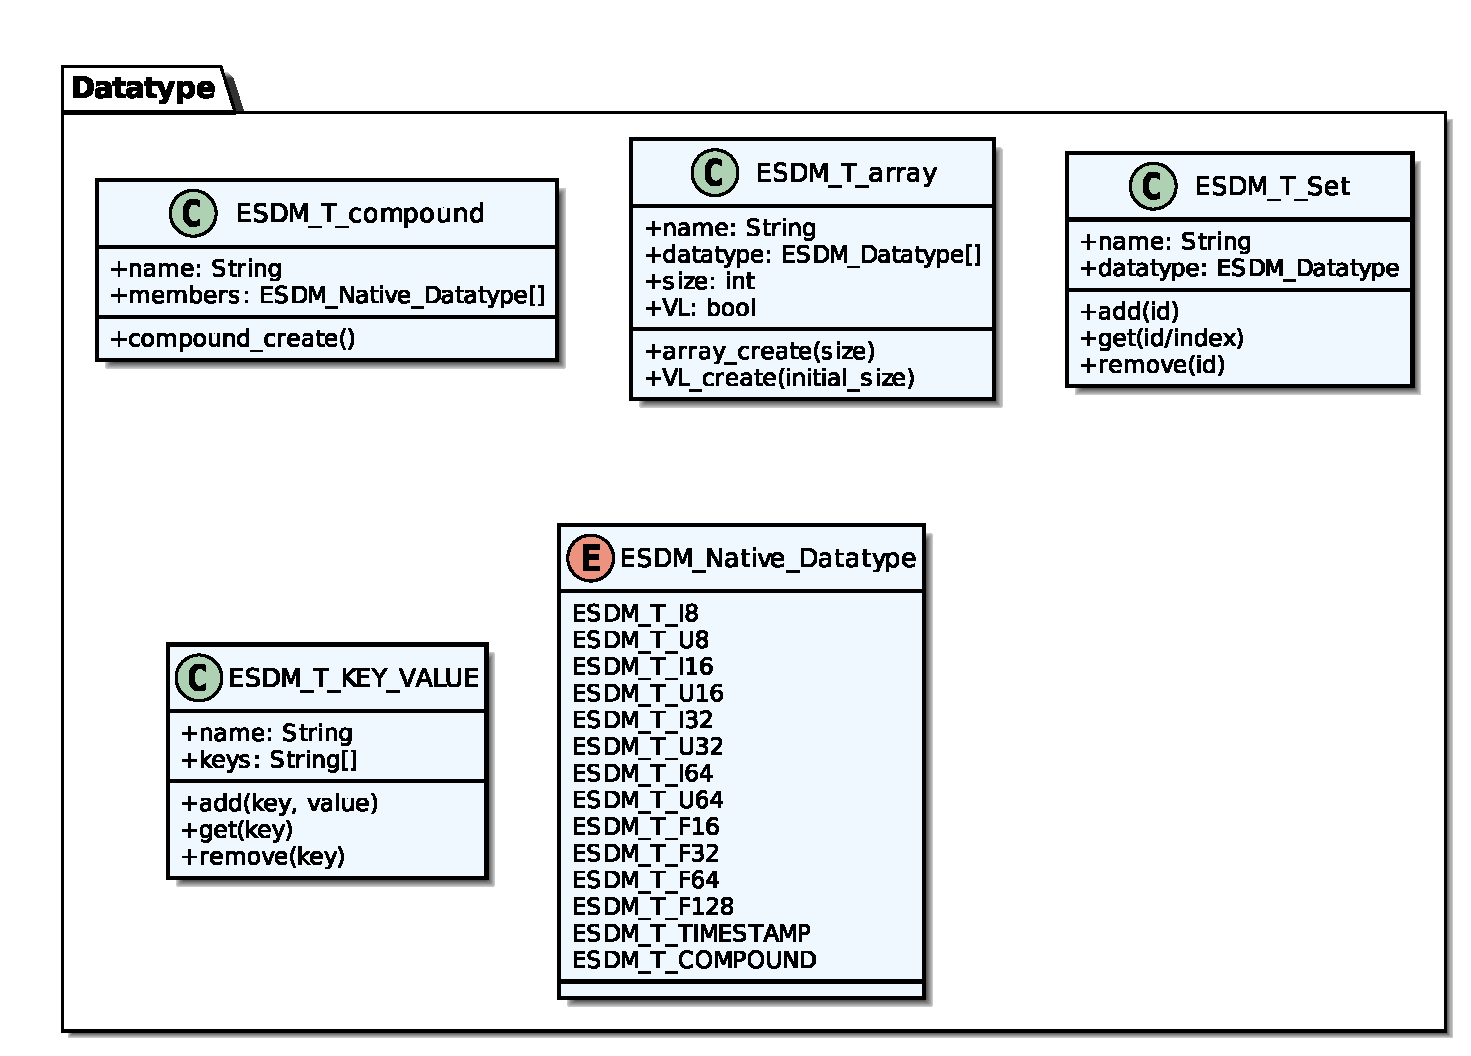
\includegraphics[width=0.9\textwidth]{esdm-semantics/semantics-datatypes.eps}
	\caption{Interfaces for the compound, array and key-value based data structures in relation to ESDM native data types.}
	\label{fig:datatypes}
\end{figure}









%%%%%%%%%%%%%
\clearpage
\section{Operations and Semantics}
\label{sec: viewpoints/logical/semantics}


\begin{figure}
	\centering
	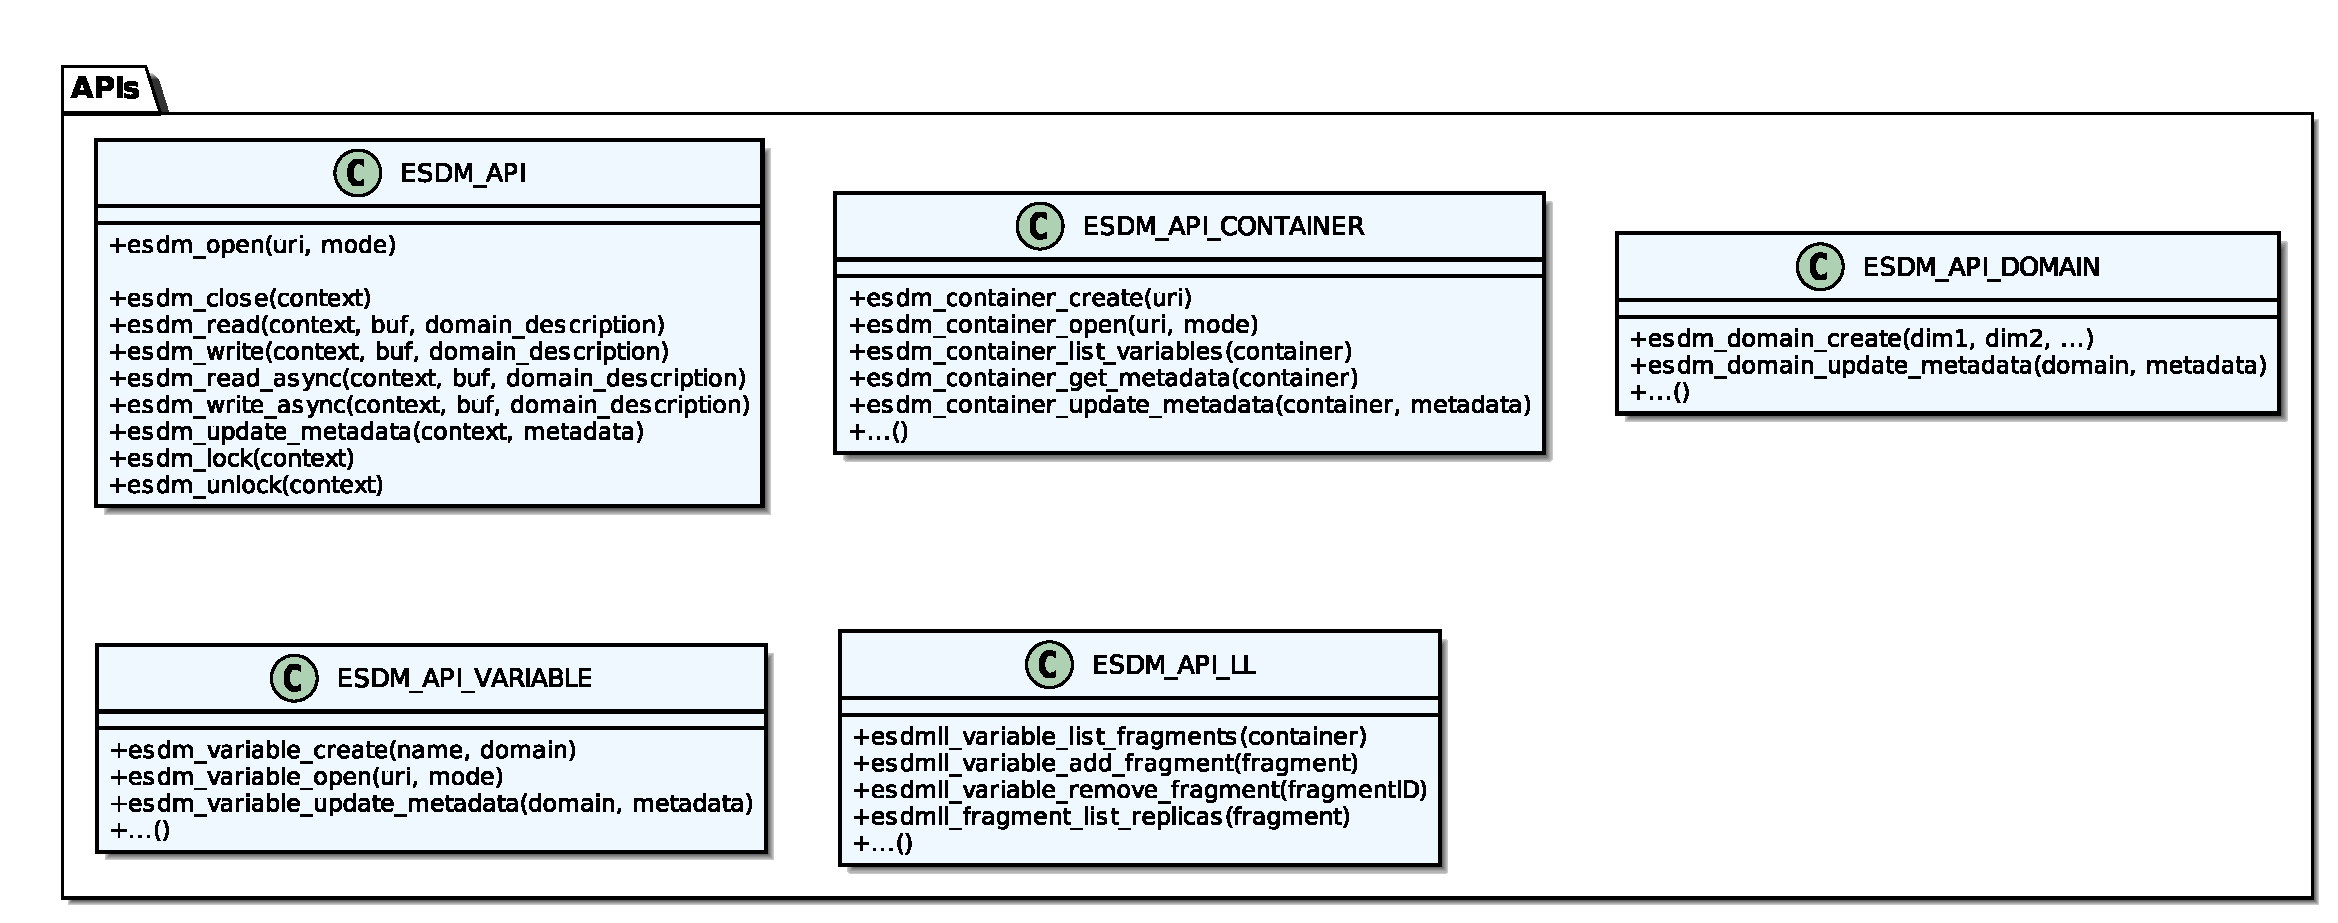
\includegraphics[width=\textwidth]{esdm-semantics/semantics.eps}
	\caption{The low and high level interfaces for standard interactions with the ESDM.}
	\label{fig:apis ll and high}
\end{figure}

This section collect the most important high-level and low-level APIs and allowed operations on ESDM data structures.
The ESDM should handle failures and many fragmentation related decisions as transparently as possible while offering a more expressive I/O API for structured data.
The conceptual model (see \Cref{subsec: conceptual data model}) does not provide the notion of files, however, some concepts familiar from file systems are also available in the ESDM system:
\begin{itemize}
\item Grouping: When existing applications are dealing with files, the ESDM will ensure that a container is available which maps onto the application view of that file.
\item Naming and Pointing: It is necessary to name things and point to them.
For a traditional file this is accomplished using a name and a file system path.
For the ESDM, we allow providing a URI which would resolve to a virtual container description or that allows to construct a virtual container on the fly linking all needed variables into it.
This is achievable because URIs are also available for all variables within a file.
\end{itemize}


\paragraph{Accessing data}

The API provides means to start reading and modification of data asynchronously and offers a \texttt{wait()} call to block until a particular operation terminates.
While the read/write is ongoing the data in memory that is read/or write must not be changed by the application, otherwise the result is undefined.

The ESDM does not support concurrent read and write scenarios, data can only be written or read (see Epoch), so the use of the ESD has one important ramification for application views of files:
\begin{itemize}
\item All interfaces which exploit the ESDM middleware will only allow file open to either read or write, but not both at the same time.
\item There can only be a single application that writes to a particular variable or fragment.
We expect that an application is using some kind of coordination mechanism to cooperate on reading and writing (more details will follow).
\item One application may write data while another reads data that has been previously written (in one previous epoch).
\end{itemize}
%\todo{Is that really what we mean?  See the todo wrt to fragment updates. This last point may need modification.}


\paragraph{Sealed Variables/Containers} ensure that data products are preserved and cannot be modified, thus URIs to these objects can typically be safely exchanged with peers.
The system may use this information to provide even more aggressive optimisations on read patterns.

\bigskip


In \Cref{fig:apis ll and high} provides an overview to the available ESDM core interfaces.
The following groups of interfaces can be distinguished:

\paragraph{Accessing existing data structures:}
ESDM data structures such as containers and variables maybe opened using an open call using a object identifier or a URI.
Likewise, it is possible to close a structure again.
A data structure has to be created before it is possible to read and write data.

\paragraph{Creation of data structures:}
The information necessary to create a ESDM data structure vary, therefore, each provides special methods to conveniently create the data structure.
It is possible to attach metadata to certain data structures such as variables and containers as they are created.


\paragraph{Exclusive access and concurrency control:}
A single parallel application may temporarily transfer own a container or variable exclusively using a locking mechanism.
This is necessary to facilitate data restructuring to rebuild upon failures or redistribute and optimise the data structures under the hood.
To allow scaling, it is sufficient that a single process of the (parallel) application maintains the lock.
Locks will timeout to prevent permanent deadlocks.
Synchronisation happens through the HDF5/MPI Vol plugin (see \Cref{frontend: hdf5 + mpi}) but may be implemented as a lightweight  library on top of MPI as well.
Any other parallel programming language should implement such a library to reduce the burden while performing certain (traditionally metadata sensitive) operations.
For efficient parallel write access, epoch semantics are available which are discussed in more detail in \Cref{sec: viewpoints/logical/data model/epochs}.
Open structures implicitly are attached with a communication channel by using events and notifications to notify upon changes in the epoch and prevent polling.
The event and notification facilities of ESDM are discussed in \Cref{sec: viewpoints/logical/data model/notification}.


\paragraph{Low level interfaces:}
In some cases, it can be more efficient to interact with the low level data structures provided by ESDM directly.
This may be the case when ESDM may not yet provide data abstractions that fit the application.
In this case developers can use the low level APIs to also access ESDM internal structures.
A direct manipulation is not possible and has to occur through an ESDM interface to ensure consistency.






%%%%%%%%%%%%%%%%%%%%%%%%%%%%%%%%%%%%
\subsection{Epoch Semantics}
\label{sec: viewpoints/logical/data model/epochs}

To allow applications developers and ESDM frontends to efficiently exploit concurrency the ESDM offers epoch semantics.
An epoch is an instant in time chosen by the parallel application.
\Cref{fig:epoch semantics} illustrates the ESDM methods to interact with epochs and also illustrates how the most recent readable view is reconstructed.
Starting with epoch 0, all processes of the parallel application participating in I/O have to agree on moving to a new epoch.
This will finalise the outstanding write requests, make the changes durable and publish the information about new data to other applications that registered to read this data.
Writing data follows the expected semantics for writes but when multiple writers update data from the same variable coordinates, i.e., they overwrite data, the result is undefined.
In fact, applications of which multiple processes write in the same epoch to the same data region are considered to be wrong.

Closing a variable or finalising ESDM will also move it to the next Epoch, thus finalise the first version.
Writing data to a variable that existed previously will overwrite the data of previous epochs.
Similarly, if a variable is opened for read/write access, the same application may now read the data from a previous epoch.
Reading data that has been written by another process of the same application (i.e., a read after write) should be prevented, as users should use means of communication inside the application to prevent this kind of access pattern.
Thus, a read request will never return the data of the current epoch but the merged perspective of all previous epochs.
In that sense, the epoch semantics is similar to the semantics of transactions but application wide and only one transaction can be active at a given time.
If a parallel application overwrites data stored in a previously by another application written variable, then this is handled similarly to a new epoch.

%\paragraph{Using epochs to identify data that must be garbage collected}
When an application crashes, only the last committed epoch remains accessible, all other data is immediately subject to garbage collection.
If an application does not use the Epoch and not finalise the ESD API correctly, then no data should become visible and durable on the storage.
%Identifying variables that need to be garbage collected is achieved by initialising the metadata for a variable with Epoch=0 and the current creation time.
%A periodic scan may identify variables that are still in Epoch 0 but were created, e.g., a day ago.




\begin{figure}
	\centering
	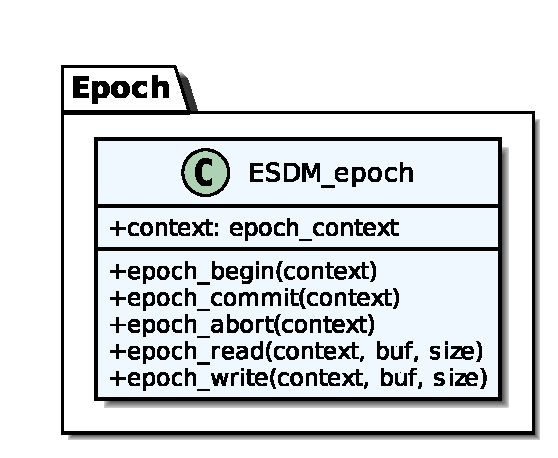
\includegraphics[width=0.38\textwidth]{esdm-semantics/semantics-epoch.eps}
	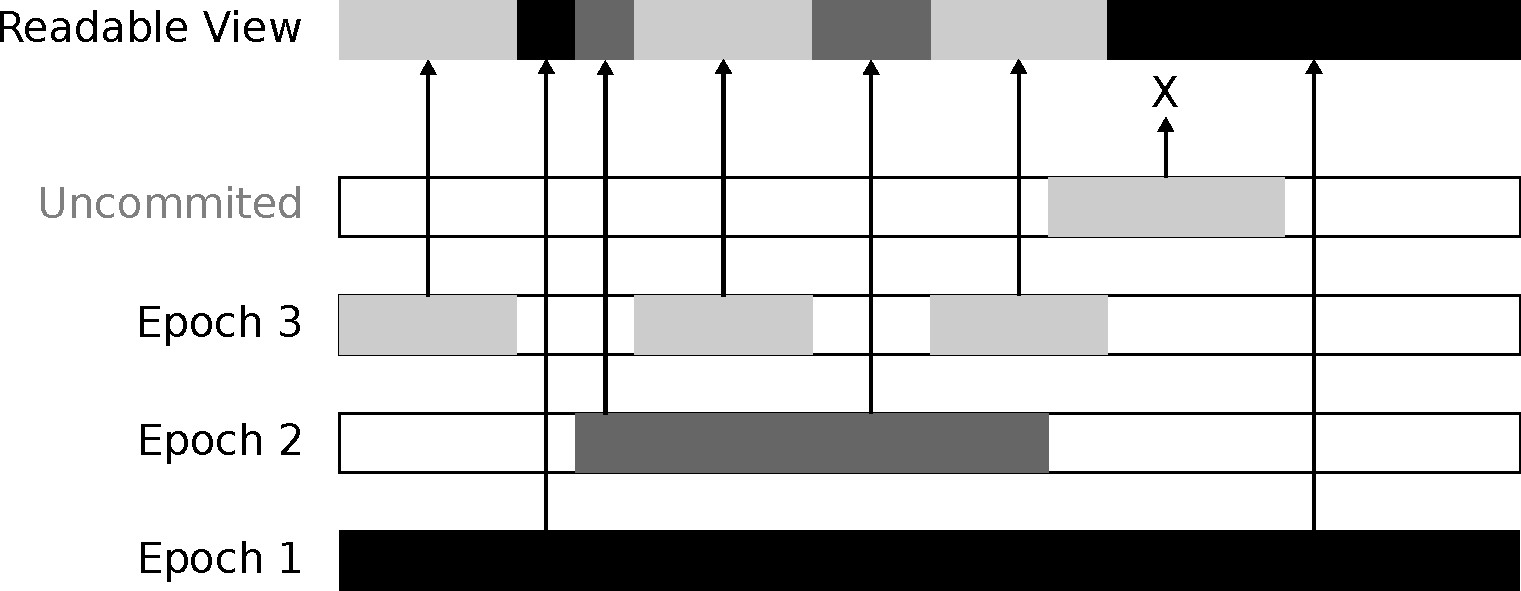
\includegraphics[width=0.6\textwidth]{esdm-semantics/epoch-reconstruction.pdf}
	\caption{Epoch API (left) and the implication of the epoch commit on the reconstruction of the most recent readable view to the data.}
	\label{fig:epoch semantics}
\end{figure}






%%%%%%%%%%%%%
\subsection{Notifications}
\label{sec: viewpoints/logical/data model/notification}

Users or software may register hooks into the ESD notification system watching for certain events to happen.
This is handled as a publish/subscribe service.
Internally, important events are logged and can be queried for the past.
This prevents loss of information in case a service is down for a period of time and ensures auditability.
Tools may use the information to monitor ongoing activity and report performance behaviour of the ESDM.
\Cref{fig:semantic notification} depicts an UML diagram for the interface to ESDM notifications.


\paragraph{Subscribe/Unsubscribe:}
A user or a process that wishes to be informed if a certain event occurs can do so by subscribing to the ESDM Notification system. If notifications are no longer necessary it can also unsubscribe again.

\paragraph{Events:}
ESDM will publish a number of standard events. \Cref{fig:semantic notification} lists a number of candidate event types.

\paragraph{User Events:}
To allow users to define workflows that depend on ESDM, users can register custom named events. Another process that is subscribed to such an event is notified when an event with the name is published.


\paragraph{Event Log:}
To allow for audits and delayed triggering of follow-up tasks in case of failures a event log is kept.
Applications and administrators may use a query interface to filter for events that are relevant.


\begin{figure}
	\centering
	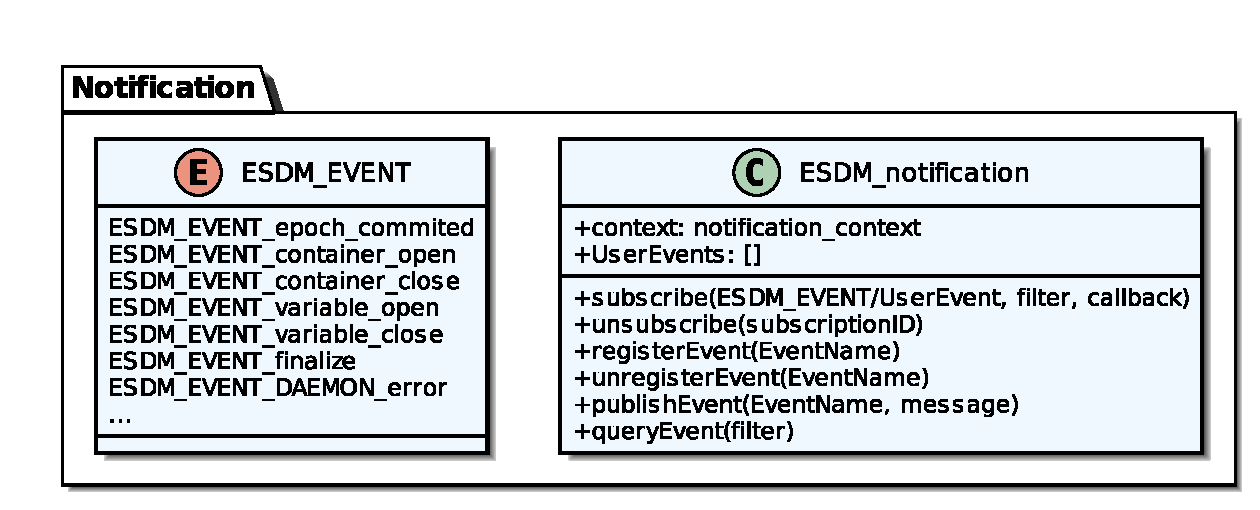
\includegraphics[width=0.8\textwidth]{esdm-semantics/semantics-notification.eps}
	\caption{Notification Interfaces and examples for possible hooks available for subscription. In addition, users may register application specific hooks.}
	\label{fig:semantic notification}
\end{figure}









%%%%%%%%%%%%%%%%%%%%%%%%%%%%%%%%%%%%%%%%%%%%%
\section{Physical view}
\label{sec: viewpoints/physical}

This section describes the relation between ESDM software components and physical hardware components such as  compute nodes, processes and the storage systems.
\Cref{fig:viewpoint physical} illustrates the interactions using UML diagrams.

\paragraph{Applications:} An application process is active on one node and may depend on multiple subcomponents.
Usually, an application will use a library such as NetCDF or HDF5 that provides a portable data description implementation.
With ESDM these libraries are slightly changed to call ESDM to handle I/O for them.
It is possible that multiple processes with ESDM are active on the same node in which case the ESDM should coordinate with processes on the same node.

\paragraph{Daemons:} Besides the application use case, a daemon process maybe necessary to ensure unreferenced fragments are cleaned up and also to perform optimisation without requiring active applications.
Multiple daemons maybe active at the same time.


\paragraph{Storage System:} Multiple storage systems maybe deployed but for the discussion the abstract representation is sufficient.
No changes to the storage backends are expected.
ESDM backends will interact with the storage systems using the interfaces that are exposed by the storage system.

\paragraph{Site Configuration:} The ESDM assumes that there is a description of the site configuration in a machine friendly format. As the system operators change the configuration of the storage systems or the network, the site configuration may need to be updated manually or automatically.




\begin{figure}
	\centering
	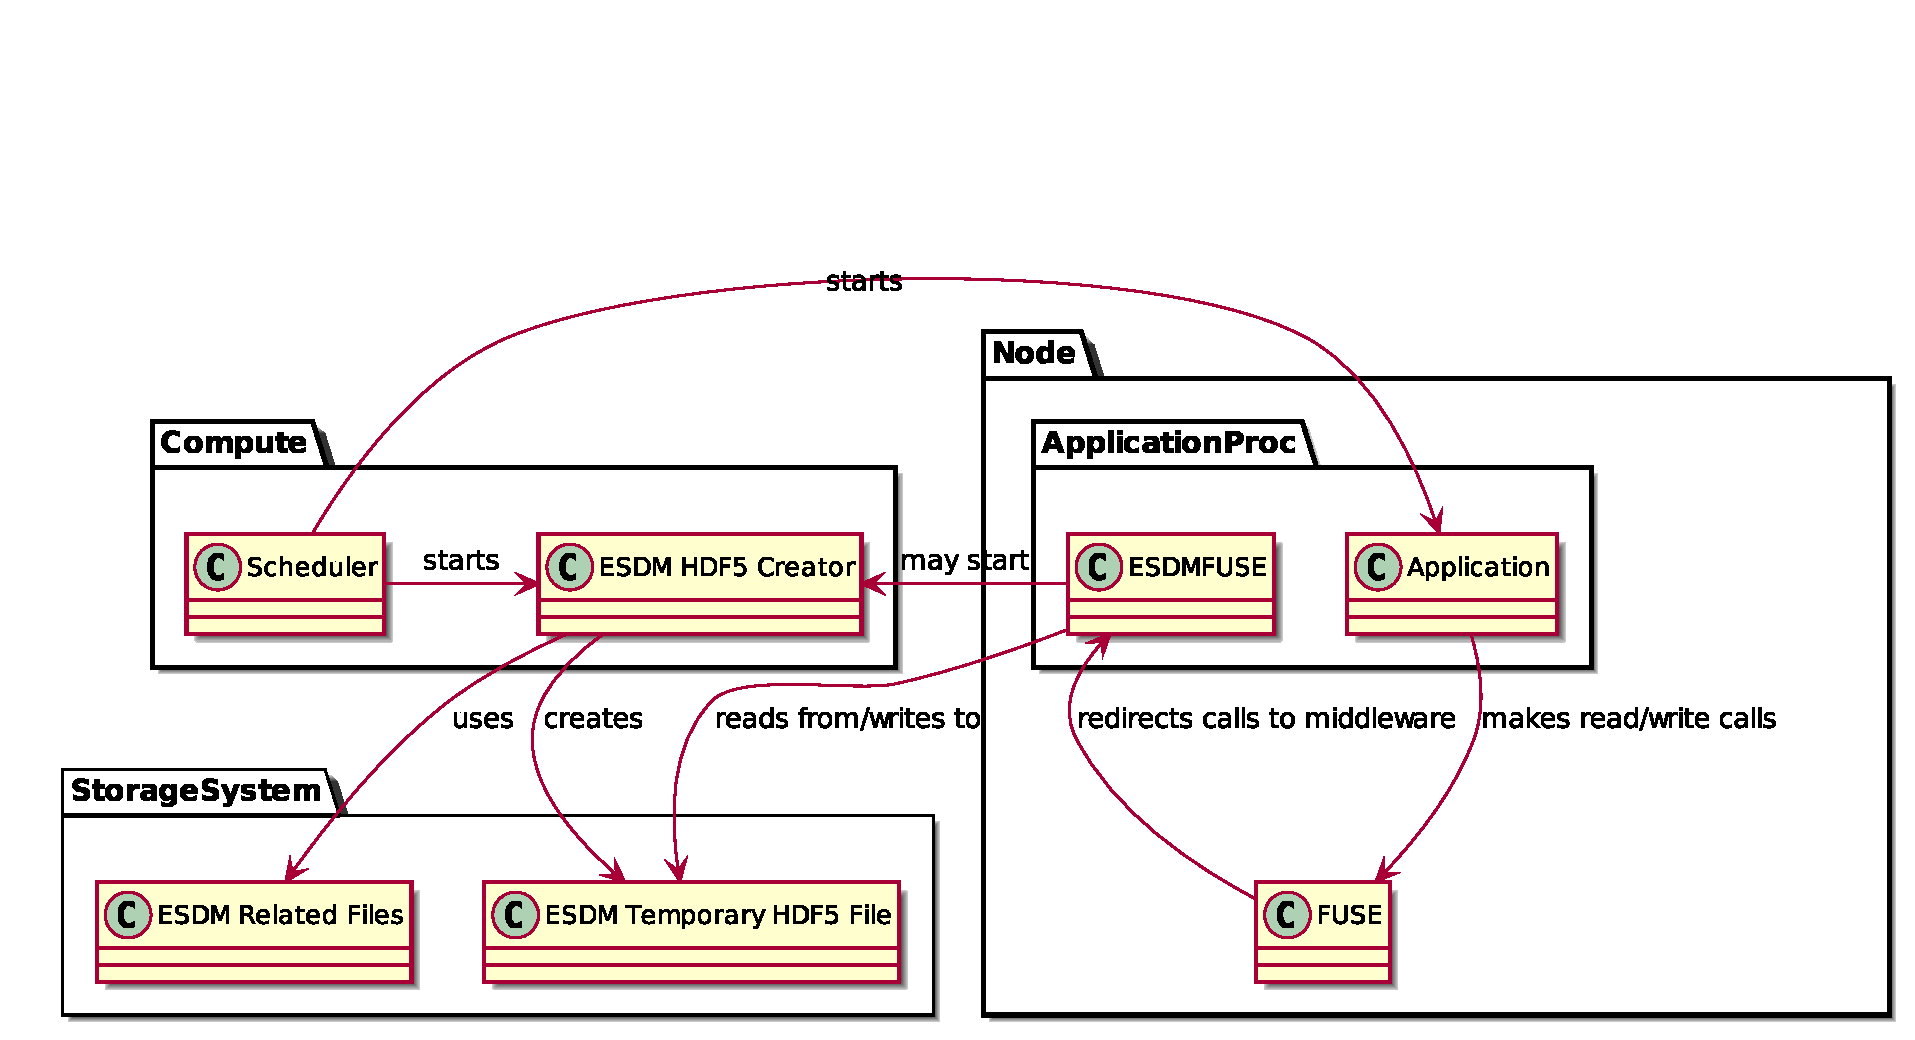
\includegraphics[width=\textwidth]{esdm/physical}
	\caption{Physical viewpoint to the core components of the ESDM.}
	\label{fig:viewpoint physical}
\end{figure}














%%%%%%%%%%%%%%%%%%%%%%%%%%%%%%%%%%%%%%%%%%%%%
\section{Process view}
\label{sec: viewpoints/process}

The process view describes active components and processes of ESDM, their interaction and how they drive the I/O.
The asynchronous I/O calls offered by ESDM still require an internal thread to progress the I/O.
Most components shown in \Cref{fig:architecture} are passive, that means functions invoked perform certain operations and return upon completion.
That means the thread of the application or tool calling ESDM retains inside ESDM until the call is completed.
The FUSE client and potential service daemons are applications in that sense, they bring their own thread that use the API of ESDM.

In the internal architecture of ESDM, the scheduler is the only exception and using threads.
Asynchronous I/O requests from user space are queued as operations to be performed by the scheduler.
% A thread of the scheduler then records the modifications to be made on a write-ahead log  => No not yet! later version
The scheduler may decide upon the order the operations are performed locally.
Internally, the scheduler hosts a queue for each storage backend that are served by a (storage backend-specific) number of threads.
A thread initiates the operation by calling the plugin-specific function.
It is the responsibility of the storage backend to ensure the data is transferred to the respective storage.
An involved storage system above of a capable network may allow RDMA.
In this case, the plugin has to announce the availability of data to the server, then the server may fetch data from the client using RDMA and send a notification upon completion.
Due to the lack of such capabilities on most storage APIs, the capabilities of pulling data is subject to a later version of ESDM.


\paragraph{ESDM daemon}

The ESDM daemon is in charge to constantly check the health of the overall system.
It will remove/garbage collect objects that were created by applications that crashed.
It may start a re-balancing/data migration between the available storage pools based on simple policies.
Also replicas of data may be removed to free space.

% \todo{figure}




\section{Requirements-Matrix}
\label{seq:req matrix}
In this section we re-visit the requirements and show how these requirements are met by some element of the architecture.
Therefore, we list the requirements in \Cref{chap:requirements} in brief and describe how they are addressed by ESDM.

\begin{enumerate}
\item CRUD-operations: The data model provides CRUD operations for the objects and in particular variables that typically hold the scientific data.
\begin{itemize}
\item Partial access: Read/write operations are supported on subdomains for a variable. Internally they may fetch data
from multiple fragments.
\end{itemize}
\item Discover, browse and list data: The ESDM namespace provides a query interface based on scientific metadata.

\item Handling of scientific/structural metadata as first class citizen: Metadata provides similar operations than data.
It can be as complex as a variable, in fact attaching a variable to another as metadata.
Internal components of ESDM are aware of the metadata.
Metadata is used for searching data but also the structural information is directly used by ESDM internally; backends make the final layout decision based on the metadata.

\item Semantical namespace: provided by the metadata queries.
\item Supporting heterogeneous storage: Backends provide plugins to predict performance of access patterns and to store/retrieve data on various storage systems.
A single variable consists of fragments that each cover a subdomain, potentially with another data layout / transformation; each fragment may reside on another backend allowing to distribute a variable across different storage technology.

\item Function shipping: this is not yet described in the design. However, the structural information about the data is a key enabler for function shipping as it allows the storage backend to understand the data structures that may then be processed.

\item Compatibility: we offer a NetCDF and HDF5 interface and a POSIX file system using FUSE.
We will explore the possibility to create data using one interface and accessing the data without data copies using another.
\end{enumerate}



These mandatory requirements are accompanied by supporting requirements:
\begin{enumerate}
\item Auditability: not described in this deliverable.
\item Configurability: ESDM provides the site configuration about available storage systems and their performance characteristics.
\item Notifications: ESDM offers a publish/subscribe interface.
\item Import/Export: This is not explicitly described in this deliverable, but a tool can be build on top of ESDM.
\item Access control: ESDM will use the available access control information but also store the ownership and permissions inside the container.
\begin{itemize}
\item Data sharing: Data sharing is at the moment limited to a site.
However, it would be easy to link a tool that uses the NetCDF interface to ESDM to enable dynamic creation of virtual containers depending on the file name (that is a query for metadata).
\end{itemize}
\end{enumerate}

The non-functional requirements are resolved as follows:
\begin{enumerate}
\item Performant: by moving the serialisation from the application into the backends and by selecting appropriate backends depending on the access patterns using the layout component and the performance model, the system should be able to make superior placement decisions and optimise layout depending on the access pattern.
\item Reliable: Fragments and variables offer methods to check for integrity (e.g., using checksums); ESDM offers replication of data, potentially transformed for performance, thus offers reliable storage.

\item Versatile: By providing a storage backend for a storage technology and a performance model, it can be integrated into ESDM.
\item User-friendly: The system hides specifics of the storage landscape and does not \textit{\textbf{require}} users to set and define technical parameters specifically to a given system.
Therewith it provides performance portable code.
\item Cost-Effective: The software will be open source, it has to be proven that it is cost effective.
\item Standards based: ESDM offers standard interfaces and uses standard interfaces for the backends, making it possible to deploy it on current systems.
\end{enumerate}

%%%%%%%%%%%%%%%%%%%%%%%%%%%%%%%%%%%%%%%%%%%%%
%\section{Development view}
%\label{sec: viewpoints/development}
%\todo{
%* internal interfaces and apis
%* how is Data Models processed internally
%* Abstract: JSON for description of Data Models info, flexible, but certain fields expected => (more details not yet determined, remains to be seen as implementation continues..)
%* How are certain operations of the Data Models implemented for manipulationen of objects within Data Model
%}
%
%
